% Options for packages loaded elsewhere
\PassOptionsToPackage{unicode}{hyperref}
\PassOptionsToPackage{hyphens}{url}
%
\documentclass[
]{book}
\usepackage{lmodern}
\usepackage{amssymb,amsmath}
\usepackage{ifxetex,ifluatex}
\ifnum 0\ifxetex 1\fi\ifluatex 1\fi=0 % if pdftex
  \usepackage[T1]{fontenc}
  \usepackage[utf8]{inputenc}
  \usepackage{textcomp} % provide euro and other symbols
\else % if luatex or xetex
  \usepackage{unicode-math}
  \defaultfontfeatures{Scale=MatchLowercase}
  \defaultfontfeatures[\rmfamily]{Ligatures=TeX,Scale=1}
\fi
% Use upquote if available, for straight quotes in verbatim environments
\IfFileExists{upquote.sty}{\usepackage{upquote}}{}
\IfFileExists{microtype.sty}{% use microtype if available
  \usepackage[]{microtype}
  \UseMicrotypeSet[protrusion]{basicmath} % disable protrusion for tt fonts
}{}
\makeatletter
\@ifundefined{KOMAClassName}{% if non-KOMA class
  \IfFileExists{parskip.sty}{%
    \usepackage{parskip}
  }{% else
    \setlength{\parindent}{0pt}
    \setlength{\parskip}{6pt plus 2pt minus 1pt}}
}{% if KOMA class
  \KOMAoptions{parskip=half}}
\makeatother
\usepackage{xcolor}
\IfFileExists{xurl.sty}{\usepackage{xurl}}{} % add URL line breaks if available
\IfFileExists{bookmark.sty}{\usepackage{bookmark}}{\usepackage{hyperref}}
\hypersetup{
  pdftitle={Sensors for Journalism},
  pdfauthor={Matt Waite},
  hidelinks,
  pdfcreator={LaTeX via pandoc}}
\urlstyle{same} % disable monospaced font for URLs
\usepackage{color}
\usepackage{fancyvrb}
\newcommand{\VerbBar}{|}
\newcommand{\VERB}{\Verb[commandchars=\\\{\}]}
\DefineVerbatimEnvironment{Highlighting}{Verbatim}{commandchars=\\\{\}}
% Add ',fontsize=\small' for more characters per line
\usepackage{framed}
\definecolor{shadecolor}{RGB}{248,248,248}
\newenvironment{Shaded}{\begin{snugshade}}{\end{snugshade}}
\newcommand{\AlertTok}[1]{\textcolor[rgb]{0.94,0.16,0.16}{#1}}
\newcommand{\AnnotationTok}[1]{\textcolor[rgb]{0.56,0.35,0.01}{\textbf{\textit{#1}}}}
\newcommand{\AttributeTok}[1]{\textcolor[rgb]{0.77,0.63,0.00}{#1}}
\newcommand{\BaseNTok}[1]{\textcolor[rgb]{0.00,0.00,0.81}{#1}}
\newcommand{\BuiltInTok}[1]{#1}
\newcommand{\CharTok}[1]{\textcolor[rgb]{0.31,0.60,0.02}{#1}}
\newcommand{\CommentTok}[1]{\textcolor[rgb]{0.56,0.35,0.01}{\textit{#1}}}
\newcommand{\CommentVarTok}[1]{\textcolor[rgb]{0.56,0.35,0.01}{\textbf{\textit{#1}}}}
\newcommand{\ConstantTok}[1]{\textcolor[rgb]{0.00,0.00,0.00}{#1}}
\newcommand{\ControlFlowTok}[1]{\textcolor[rgb]{0.13,0.29,0.53}{\textbf{#1}}}
\newcommand{\DataTypeTok}[1]{\textcolor[rgb]{0.13,0.29,0.53}{#1}}
\newcommand{\DecValTok}[1]{\textcolor[rgb]{0.00,0.00,0.81}{#1}}
\newcommand{\DocumentationTok}[1]{\textcolor[rgb]{0.56,0.35,0.01}{\textbf{\textit{#1}}}}
\newcommand{\ErrorTok}[1]{\textcolor[rgb]{0.64,0.00,0.00}{\textbf{#1}}}
\newcommand{\ExtensionTok}[1]{#1}
\newcommand{\FloatTok}[1]{\textcolor[rgb]{0.00,0.00,0.81}{#1}}
\newcommand{\FunctionTok}[1]{\textcolor[rgb]{0.00,0.00,0.00}{#1}}
\newcommand{\ImportTok}[1]{#1}
\newcommand{\InformationTok}[1]{\textcolor[rgb]{0.56,0.35,0.01}{\textbf{\textit{#1}}}}
\newcommand{\KeywordTok}[1]{\textcolor[rgb]{0.13,0.29,0.53}{\textbf{#1}}}
\newcommand{\NormalTok}[1]{#1}
\newcommand{\OperatorTok}[1]{\textcolor[rgb]{0.81,0.36,0.00}{\textbf{#1}}}
\newcommand{\OtherTok}[1]{\textcolor[rgb]{0.56,0.35,0.01}{#1}}
\newcommand{\PreprocessorTok}[1]{\textcolor[rgb]{0.56,0.35,0.01}{\textit{#1}}}
\newcommand{\RegionMarkerTok}[1]{#1}
\newcommand{\SpecialCharTok}[1]{\textcolor[rgb]{0.00,0.00,0.00}{#1}}
\newcommand{\SpecialStringTok}[1]{\textcolor[rgb]{0.31,0.60,0.02}{#1}}
\newcommand{\StringTok}[1]{\textcolor[rgb]{0.31,0.60,0.02}{#1}}
\newcommand{\VariableTok}[1]{\textcolor[rgb]{0.00,0.00,0.00}{#1}}
\newcommand{\VerbatimStringTok}[1]{\textcolor[rgb]{0.31,0.60,0.02}{#1}}
\newcommand{\WarningTok}[1]{\textcolor[rgb]{0.56,0.35,0.01}{\textbf{\textit{#1}}}}
\usepackage{longtable,booktabs}
% Correct order of tables after \paragraph or \subparagraph
\usepackage{etoolbox}
\makeatletter
\patchcmd\longtable{\par}{\if@noskipsec\mbox{}\fi\par}{}{}
\makeatother
% Allow footnotes in longtable head/foot
\IfFileExists{footnotehyper.sty}{\usepackage{footnotehyper}}{\usepackage{footnote}}
\makesavenoteenv{longtable}
\usepackage{graphicx,grffile}
\makeatletter
\def\maxwidth{\ifdim\Gin@nat@width>\linewidth\linewidth\else\Gin@nat@width\fi}
\def\maxheight{\ifdim\Gin@nat@height>\textheight\textheight\else\Gin@nat@height\fi}
\makeatother
% Scale images if necessary, so that they will not overflow the page
% margins by default, and it is still possible to overwrite the defaults
% using explicit options in \includegraphics[width, height, ...]{}
\setkeys{Gin}{width=\maxwidth,height=\maxheight,keepaspectratio}
% Set default figure placement to htbp
\makeatletter
\def\fps@figure{htbp}
\makeatother
\setlength{\emergencystretch}{3em} % prevent overfull lines
\providecommand{\tightlist}{%
  \setlength{\itemsep}{0pt}\setlength{\parskip}{0pt}}
\setcounter{secnumdepth}{5}
\usepackage{booktabs}
\usepackage{amsthm}
\makeatletter
\def\thm@space@setup{%
  \thm@preskip=8pt plus 2pt minus 4pt
  \thm@postskip=\thm@preskip
}
\makeatother
\usepackage[]{natbib}
\bibliographystyle{apalike}

\title{Sensors for Journalism}
\author{Matt Waite}
\date{2020-06-18}

\begin{document}
\maketitle

{
\setcounter{tocdepth}{1}
\tableofcontents
}
\hypertarget{introduction}{%
\chapter*{Introduction}\label{introduction}}
\addcontentsline{toc}{chapter}{Introduction}

Most of the data journalism done throughout the world uses data collected by the government. The problem with that is twofold: That means data journalists are reliant upon the government to do their journalism, and what happens when the government doesn't collect the data.

There are ways for journalists to create their own data -- surveys, keying in data from documents or, for well funded organizations, hiring workers to collect it. Another way, which is lightly explored but potentially powerful, is using off-the-shelf sensors to collect that data.

Some major milestone projects for sensors in journalism:

\begin{itemize}
\tightlist
\item
  \href{https://project.wnyc.org/cicadas/}{Cicada Tracker}: A WNYC project that made ground temperature sensors and a means for people to report that temperature to track the emergence of 17-year cicadas. Hundreds of volunteers built sensors and reported data to the project in 2013.
\item
  \href{https://inewsource.org/whats-in-the-air/}{What's in the Air?}: The School of Journalism and Media Studies at San Diego State University used air quality sensors to report on air pollution in their city in 2014-2015.
\item
  \href{https://cnsmaryland.org/interactives/summer-2019/code-red/behind-scenes.html}{Code Red}: The University of Maryland's Philip Merrill College of Journalism partnered with NPR to report on inequality in climate change, specifically measuring differences in temperatures inside people's houses. They built temperature and humidity sensors to show what it's like to live in Baltimore's rowhouses during a hot summer.
\end{itemize}

What all three projects combine is some simple electronics, inexpensive sensors, basic programming and a giant bucket of creativity. The electronics and the programming are within reach of anyone willing to take the time to learn.

The creativity is the hard part.

What follows is an introduction to the electronics and programming parts of that equation. The creativity part is entirely up to you. The more you can think about how to apply these ideas, the better chance you have of finding that creative spark.

\hypertarget{what-to-buy}{%
\section{What to buy}\label{what-to-buy}}

The truth is this is an impossible question to ask because of several factors.
1. You will have your own ideas of what you're going to want to do, and that will drive your decisions.
2. The technology available changes constantly and at a breathtaking pace.
3. The programming languages that glue this all together also change, albeit less quickly.

So what follows is an attempt to suggest things that could cover a wide variety of applications, but have been specifically chosen for this book and the project described in later chapters.

\textbf{If you are planning an introductory classroom based course:} The first half of this book uses the \href{https://www.adafruit.com/product/3333}{Circuit Playground Express}. It's an excellent, all-in-one beginner board that has a ton of features on it: lights, sensors, and can be programmed multiple ways. In a single board, you can program it with a visual, web-based interface from Microsoft called MakeCode that's largely aimed at kids and you can program it with Circuit Python. This is great for students who have no experience with code: You can use MakeCode to do drag-and-drop programming to show what you can do and then switch to code to make the transition from the real to the abstract a smoother ride. There is a \href{https://www.adafruit.com/product/3399}{Circuit Playground Express Educator's Pack} that gets you 15 boards, 15 USB cables and some fun extras for, at the time of this writing, \$350.

\textbf{If you are planning a project}: For project work, you are going to want more flexibility in a smaller form factor. For this book, we're going to use the Adafruit Feather series, specifically the \href{https://www.adafruit.com/product/4516}{Adafruit Feather Sense}, which packs a sensor array similar to the Circuit Playground Express, and we're going to add the \href{https://www.adafruit.com/product/2922}{Adalogger FeatherWing}, an add on to give us a real time clock and an microSD card reader for data logging. For that we get sensors, clock, data logging and external power management for \$38 a board. Could you do this cheaper by buying separate sensors and building this yourself? Without question. But it would be difficult and time consuming for beginners. Time is money.

\hypertarget{why-circuit-python}{%
\section{Why circuit python?}\label{why-circuit-python}}

This is largely personal opinion, but there's a solid argument here.

\begin{enumerate}
\def\labelenumi{\arabic{enumi}.}
\tightlist
\item
  Arduino has been the most visible small electronics platform for years and years. The one knock on it? It's based in C, which is an especially difficult language for beginners to learn.
\item
  Python is one of, if not the fastest growing programming language in the world right now. There's reasons beyond this project for students to learn Python.
\item
  Python is one of the more beginner friendly languages to learn. The syntax is largely straightforward and the fiddly parts are manageable with practice.
\item
  It is much easier to see what your code is doing in Python versus the old Arduino code.
\end{enumerate}

The downsides to using Circuit Python, in the interest of fairness:

\begin{itemize}
\tightlist
\item
  Micro Python, and the Circuit Python variant, are relatively new.
\item
  The main consequences of that newness are that there's years and years of code, message board and tutorial support for Arduino out there and there just isn't that for Circuit Python \ldots{} yet.
\item
  There's fewer options for boards that support Circuit/Micro Python.
\end{itemize}

On balance, I believe the benefit of students learning some Python outweighs the downsides. Especially if this is the only chance they'll have to learn a programming language. Connecting code to the physical world is a powerful way to learn it.

\hypertarget{setup}{%
\chapter{Setup}\label{setup}}

The first step of any sensor journalism project is setting up your environment.

It is, unfortunately, a moving target. Fortunately, Adafruit keeps updated instructions available.

\textbf{Windows Users}: \href{https://learn.adafruit.com/adafruit-circuit-playground-express/adafruit2-windows-driver-installation}{You will need to first install drivers}.

\textbf{All Users}: \href{https://learn.adafruit.com/adafruit-circuit-playground-express/updating-the-bootloader}{You may to update the bootloader}, especially if you are on a Mac.

\hypertarget{first-things-first}{%
\section{First things first}\label{first-things-first}}

Let's have some fun.

Plug in your Circuit Playground to a USB port on your computer. You should see two things happen: first, your LEDs should all turn green like this:

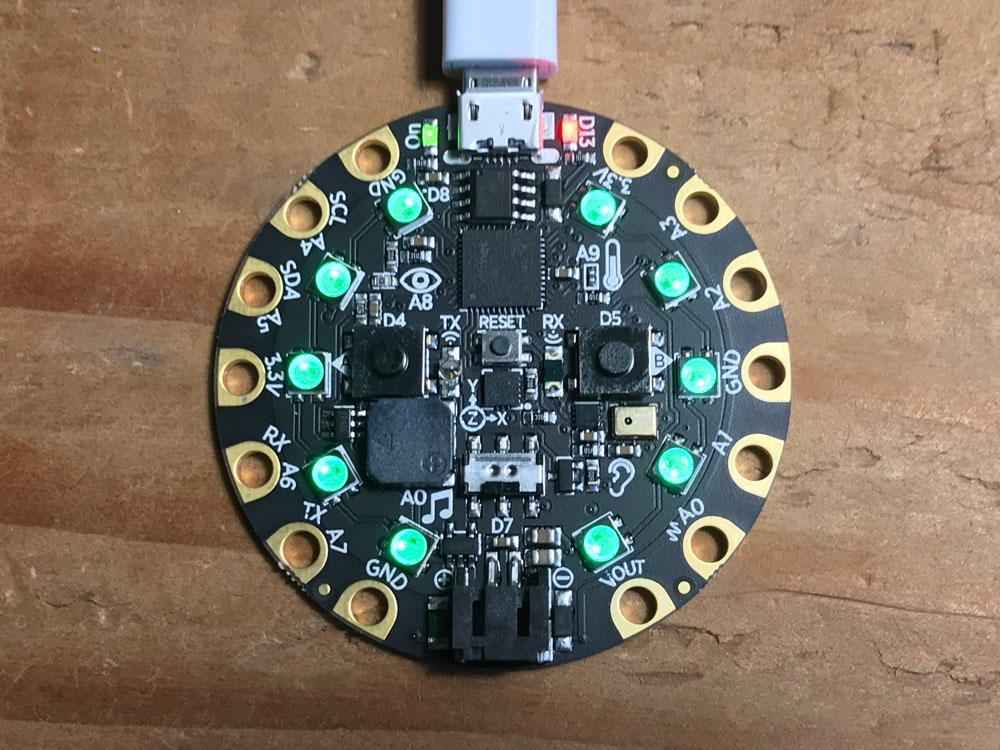
\includegraphics[width=1\linewidth]{images/01image1}

And you should now have a USB drive on your computer called CPLAYBOOT.

If that's the case, you're good to go. If not, review the Adafruit setup instructions.

Let's go to the \href{https://makecode.adafruit.com/}{MakeCode site specifically for the Circuit Playground Express}.

Click on the big blue New Project box.

You should get a workspace, with concepts you can work with on the left, and the execution space on the right, with a U shaped box that ominously says ``forever'' on it.

In this workspace, you can drag commands into the space, arrange them, and execute them on your board. To demonstrate, let's click on the Light box and drag out the ``show animation for 500 ms'' bar into the workspace. Then, drag it into the forever box so they snap together.

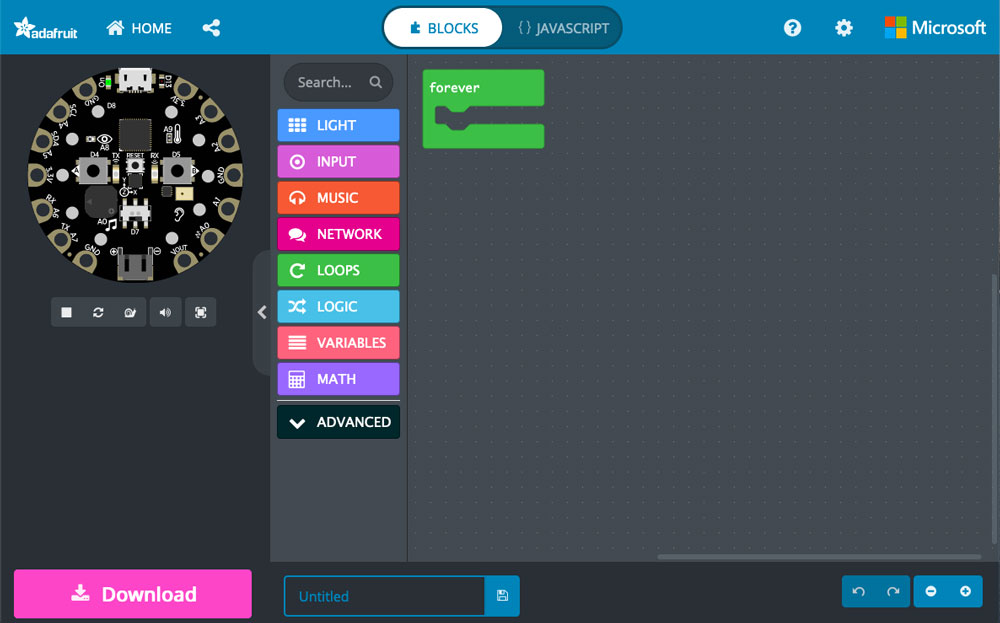
\includegraphics[width=1\linewidth]{images/01image2}

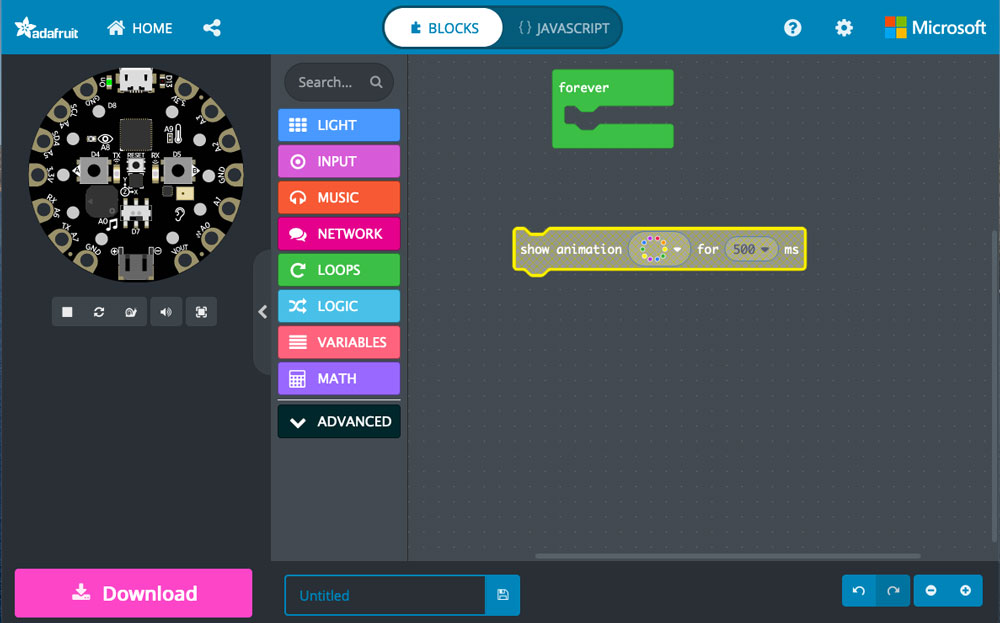
\includegraphics[width=1\linewidth]{images/01image3}

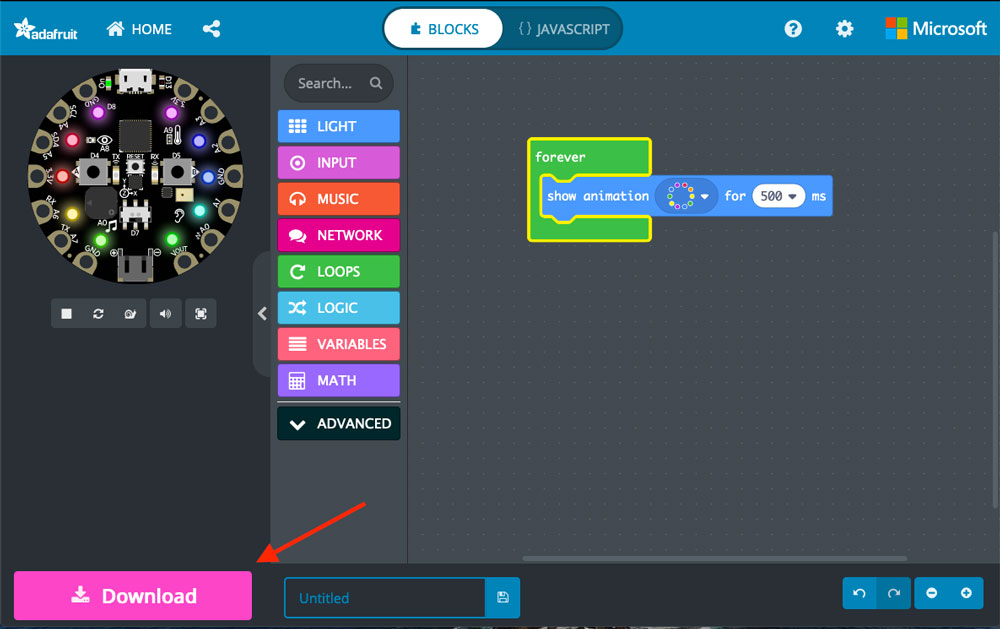
\includegraphics[width=1\linewidth]{images/01image4}

Then, click the Download button. The code to run on your board will download to your Downloads folder with a .uf2 extension on it. Drag that file into your CPLAYBOOT drive. When that happens, CPLAYBOOT is going to disappear (and on a Mac, you'll get that dreaded Disk Not Ejected Properly warning that you can, in this case, completely ignore).

What's your Circuit Playground Express doing? Is it spinning a rainbow at you over and over?

Congratulations, you're a hardware programmer.

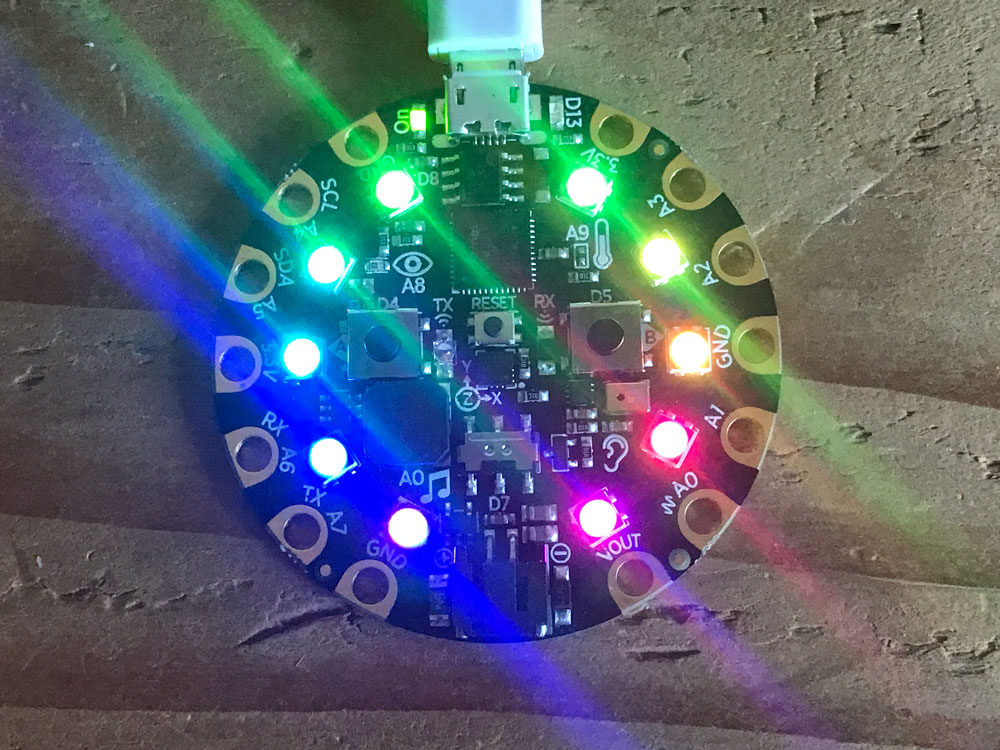
\includegraphics[width=1\linewidth]{images/01image5}

\hypertarget{installing-circuit-python}{%
\section{Installing Circuit Python}\label{installing-circuit-python}}

Your Circuit Playground is capable of running both MakeCode and Circuit Python. To install Circuit Python, you'll need to follow a few steps:

\begin{enumerate}
\def\labelenumi{\arabic{enumi}.}
\tightlist
\item
  \href{https://learn.adafruit.com/adafruit-circuit-playground-express/circuitpython-quickstart}{Install the latest version of Circuit Python on your board}.
\item
  \href{https://learn.adafruit.com/adafruit-circuit-playground-express/installing-mu-editor}{Install mu-editor, a simple and free code editor for Circuit Python}.
\end{enumerate}

Once you've got that going, time to look at some Python basics.

\hypertarget{python-basics}{%
\chapter{Python basics}\label{python-basics}}

Python is a great language to learn if you've never seen code before, or if you have little experience with it. With a little bit of practice, you can get to reading someone else's Python code and have a decent idea of what it is doing. There is a lot of code to borrow on the internet, and a fair number of times you can find what you need on a site or a message board.

But the copy and pray method of development is not a good plan. Better to learn some basics and grow into some knowledge.

The basics that you need to get started with Python -- and by extension, Circuit Python -- are:

\begin{enumerate}
\def\labelenumi{\arabic{enumi}.}
\tightlist
\item
  Variables
\item
  Functions
\item
  Loops
\item
  Conditionals
\item
  Error trapping
\item
  Libraries.
\end{enumerate}

It's just six things, and we'll go through each one here. As we go forward with making your board do things, we'll highlight these concepts and how most of what we're doing is just mixing them around in new and creative ways.

In the last chapter, you installed mu-editor. Open mu-editor, then click on Mode and choose Python 3.

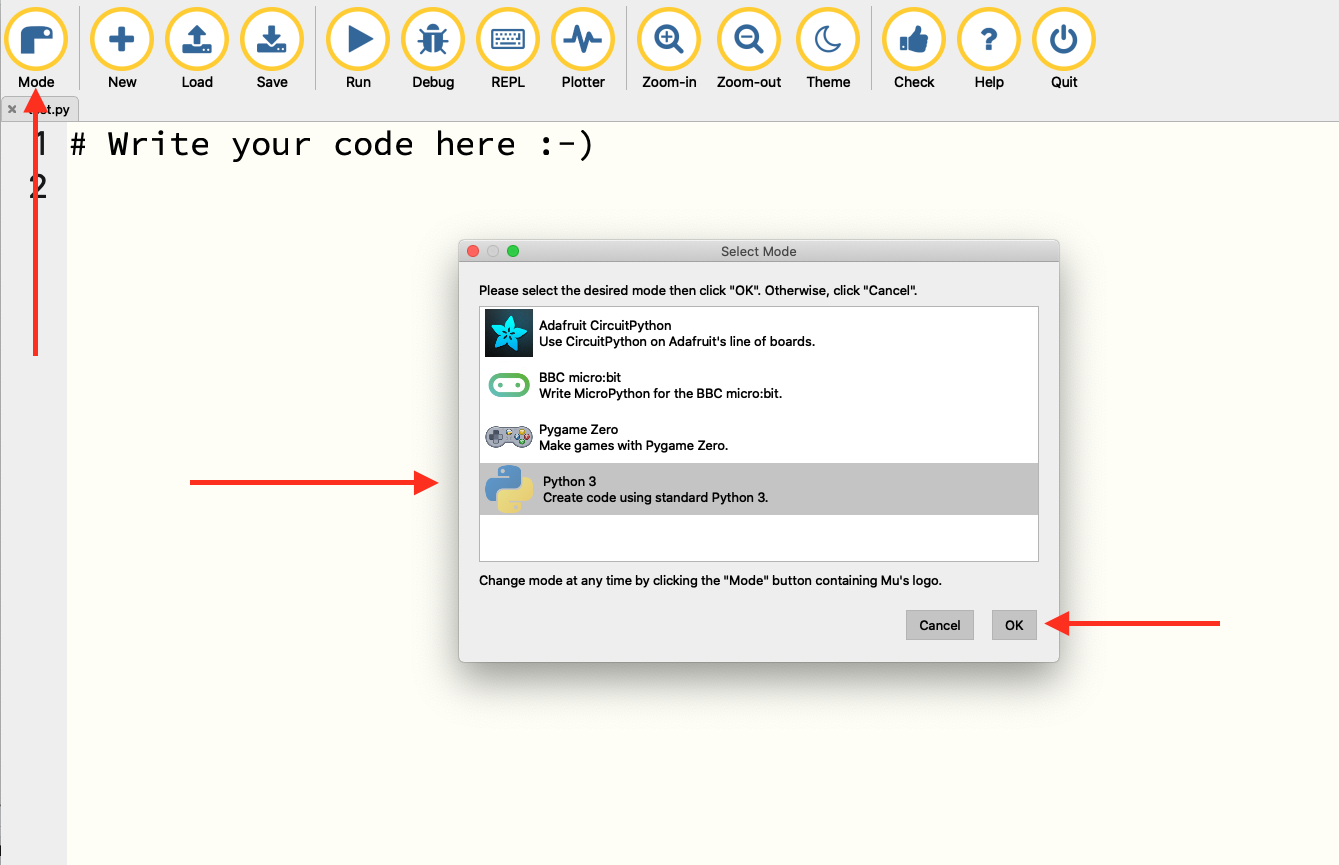
\includegraphics[width=1\linewidth]{images/02image1}

Then, just click the Run button.

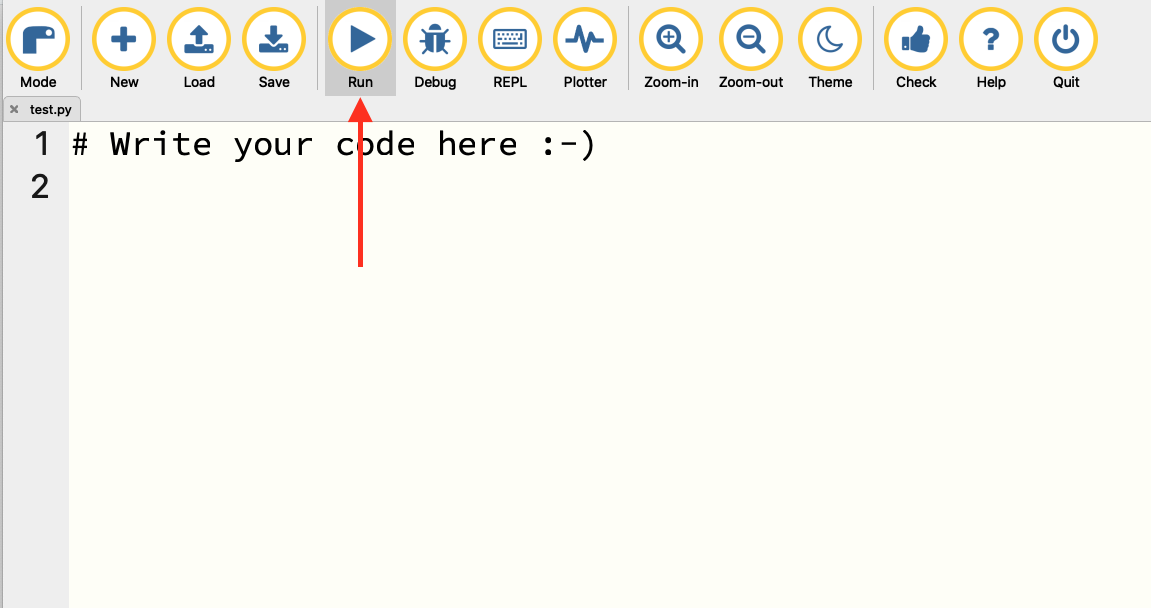
\includegraphics[width=1\linewidth]{images/02image2}

That should pop up a pane at the bottom of your window like this:

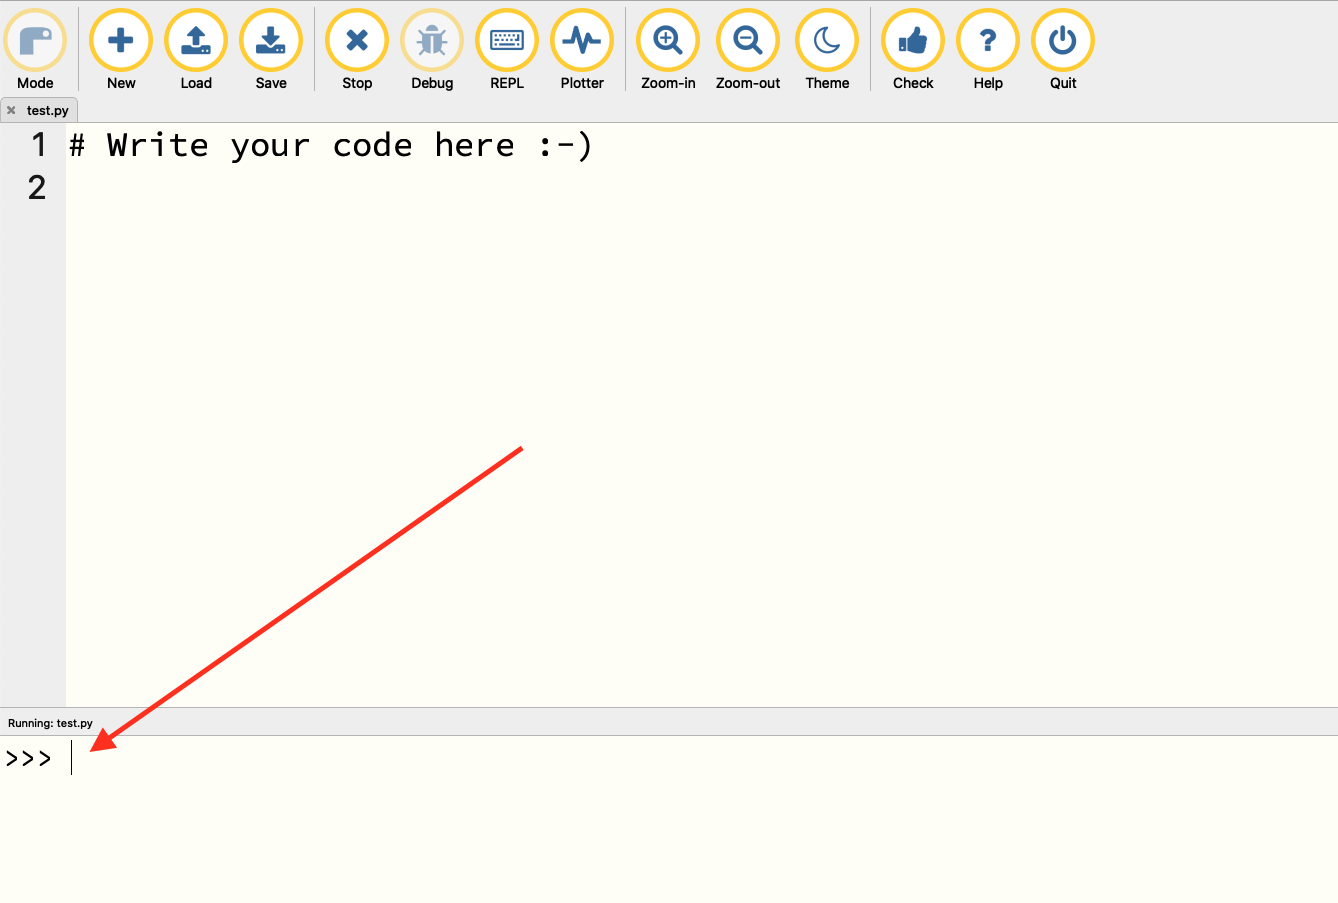
\includegraphics[width=1\linewidth]{images/02image3}
In that pane, next to the \texttt{\textgreater{}\textgreater{}\textgreater{}} you'll be able to just type Python code and execute it. So let's try some.

\hypertarget{variables}{%
\section{Variables}\label{variables}}

One of your first lessons is to not make things more complicated than you need. If you've been told that programming is hard, the truth is it can be, but it doesn't have to be. And if you've been told that things are highly technical and you wouldn't understand them, that's a lie.

Most of programming is very simple. The complexity comes in what we want to do and how those things mix together. Fortunately for us, most of what we want to do is simple, using simple concepts and easy to understand ideas.

The variable is your first lesson in simple.

A variable is just a thing that stores stuff. That's it. It could be a number. Or some text. It could be a whole list of numbers, the entire text of War and Peace, or every reading from one of our sensors. It can be anything in our computers, or on someone else's in some cases.

Here's where variables come into play.

First, python can act like a calculator. We can just add two numbers together. Try this in your terminal.

\begin{Shaded}
\begin{Highlighting}[]
\DecValTok{2} \OperatorTok{+} \DecValTok{2}
\end{Highlighting}
\end{Shaded}

\begin{verbatim}
## 4
\end{verbatim}

Simple, right? We know the answer to this before we run it and, sure enough, Python gives us the right answer.

But what if we want to store the result of that math to use later? We use a variable. And in Python, variables are created with an equal sign. Type this in your terminal and hit enter.

\begin{Shaded}
\begin{Highlighting}[]
\NormalTok{number }\OperatorTok{=} \DecValTok{2} \OperatorTok{+} \DecValTok{2} 
\end{Highlighting}
\end{Shaded}

Uh oh. Seems like nothing happend, right? We typed something and we got nothing. Well, let this be another lesson -- code does exactly what you tell it to do, not what you want it to do. In this case, we told it to store 2 + 2 into a variable called number. We didn't say show us the number. We didn't say anything else. Just store it.

Want to see it? Type this an hit enter:

\begin{Shaded}
\begin{Highlighting}[]
\BuiltInTok{print}\NormalTok{(number)}
\end{Highlighting}
\end{Shaded}

\begin{verbatim}
## 4
\end{verbatim}

This does what you think it does. It prints out (to the screen) your variable. This is really a function, which we'll discuss in a bit, but any time you want to see the thing you're working with, just print it.

In Python, how things like variables are formatted matters. Notice our numbers are just numbers: \texttt{2}. A number, without any quotation marks, is automatically formatted as a number. To automatically format something as text, you put it in quotes. Type this:

\begin{Shaded}
\begin{Highlighting}[]
\BuiltInTok{print}\NormalTok{(}\StringTok{"I am learning Python"}\NormalTok{)}
\end{Highlighting}
\end{Shaded}

\begin{verbatim}
## I am learning Python
\end{verbatim}

What happens if you don't put it in quotes?

\begin{Shaded}
\begin{Highlighting}[]
\BuiltInTok{print}\NormalTok{(I am learning Python)}
\end{Highlighting}
\end{Shaded}

You get an invalid syntax error. That's because without the quotes, Python thinks I, am, learning and Python are variable names.

Where this gets hard is numbers that aren't numbers. We looked at something simple like \texttt{2+2}. But what happens when you have a zip code? Is a zip code a number? The answer is no -- you would never do math with a zip code. So \texttt{2} is a number, \texttt{"2"} is text. What happens if you try to add text together?

\begin{Shaded}
\begin{Highlighting}[]
\CommentTok{"2"} \OperatorTok{+} \StringTok{"2"} 
\end{Highlighting}
\end{Shaded}

\begin{verbatim}
## '22'
\end{verbatim}

If your reaction is \ldots{} uh, what? \ldots{} there's something you need to know. In Python, \texttt{+} between two numbers means add, but \texttt{+} between two pieces of text means merge these two pieces of text together. So first -- see that \texttt{"2"+"2"} equals \texttt{\textquotesingle{}22\textquotesingle{}}. But see the single quote marks around them? That means that \texttt{22} is really \texttt{"22"} or text, not a number.

\hypertarget{functions}{%
\section{Functions}\label{functions}}

You've already used a function when you printed something out. The definition of a function is a piece of code that takes input and returns output. That's it. Input. Output. Your \texttt{print()} function took in your variable and printed it out.

The basic rule of thumb on functions is that if you are going to do it twice, you should make it a function. Let's make a simple function to convert Celsius to Fahrenheit. To convert Celsius to Fahrenheit, you take your number, multiply it by 1.8 and then add 32. We can do this with a calculator easily. Some of you might be able to do it in your head. But what if you wanted to do it every 10 seconds? You want a function.

To create a function, you define it with \texttt{def}, give it a name, and then name your input value.

\begin{quote}
\textbf{An important note about Python:} Python has what is called Meaningful White Space, meaning indentations matter. Code that is indented under code that isn't indented is considered part of that code -- a continuation of it. Then, when the code returns to not being indented again, the block of code is considered done. **In Python, indentations are made with four spaces, NOT tabs.
\end{quote}

Our function will create a variable called \texttt{fahren}, short for Fahrenheit, and then do the math. Our output will print the Fahrenheit value.

\begin{Shaded}
\begin{Highlighting}[]
\KeywordTok{def}\NormalTok{ convert(temp):}
\NormalTok{    fahren }\OperatorTok{=}\NormalTok{ (temp }\OperatorTok{*} \FloatTok{1.8}\NormalTok{) }\OperatorTok{+} \DecValTok{32} \CommentTok{# note the four spaces}
    \BuiltInTok{print}\NormalTok{(fahren) }\CommentTok{# note the four spaces}
\end{Highlighting}
\end{Shaded}

Now, to use it, we can just call \texttt{convert} and give it a number. What is 28 Celsius in Fahrenheit?

\begin{Shaded}
\begin{Highlighting}[]
\NormalTok{convert(}\DecValTok{28}\NormalTok{)}
\end{Highlighting}
\end{Shaded}

\begin{verbatim}
## 82.4
\end{verbatim}

So 28 Celsius is 82.4 Fahrenheit. A nice warm day.

Later, we'll explore functions that other people have made for us when we talked about external libraries. The important things to remember -- functions take input and provide output.

\hypertarget{loops}{%
\section{Loops}\label{loops}}

Loops are the most powerful feature in programming. Just about every website and app that you use in a day are, at their core, a loop. Loops repeat a series of commands on a piece of data until either there is no more data to work with or, in some cases, forever. For example, let's use Instagram. When you log into Instagram, a request goes to Facebook's servers and gets the latest photos from your friends and the people you follow. Those photos are then put into a list. Your list might have a few new photos or it may have hundreds. We don't know until we look. Then, on your phone, those photos appear, one after another, until the list runs out (when another request is fired off, bringing you more photos in an attempt to keep you there longer).

That's a loop.

So first, let's create a list of Celsius readings. Lists in Python are created with brackets:

\begin{Shaded}
\begin{Highlighting}[]
\NormalTok{myreadings }\OperatorTok{=}\NormalTok{ [}\FloatTok{20.2}\NormalTok{, }\FloatTok{20.8}\NormalTok{, }\FloatTok{21.1}\NormalTok{, }\FloatTok{20.9}\NormalTok{, }\FloatTok{20.7}\NormalTok{]}
\end{Highlighting}
\end{Shaded}

One of the most beginner friendly parts of Python is the simplicity of loops. When you see it, you can pretty much read it right away. There's two kinds of loops. Let's start with the \texttt{for} loop. In English, what Python's \texttt{for} loop code is saying is this: For each instance of a thing in a list of things, do this. Here's what that looks like in code:

\begin{Shaded}
\begin{Highlighting}[]
\ControlFlowTok{for}\NormalTok{ reading }\KeywordTok{in}\NormalTok{ myreadings:}
    \BuiltInTok{print}\NormalTok{(reading)}
\end{Highlighting}
\end{Shaded}

\begin{verbatim}
## 20.2
## 20.8
## 21.1
## 20.9
## 20.7
\end{verbatim}

The first parts of that code -- reading -- can be anything we want it to be.

\begin{Shaded}
\begin{Highlighting}[]
\ControlFlowTok{for}\NormalTok{ thereisnoplacelikenebraska }\KeywordTok{in}\NormalTok{ myreadings:}
    \BuiltInTok{print}\NormalTok{(thereisnoplacelikenebraska)}
\end{Highlighting}
\end{Shaded}

\begin{verbatim}
## 20.2
## 20.8
## 21.1
## 20.9
## 20.7
\end{verbatim}

The second part -- allofmyreadings -- is our list that we created. The second part must exist somewhere before we run the loop. A good coding habit to get into? Name things what they are. Don't get cute. And don't create things difficult to spell. Don't name things single letters. Give it a real name. So the first example is good, the second example, while dear to my heart, is bad.

So now we can combine our function and our loop.

\begin{Shaded}
\begin{Highlighting}[]
\ControlFlowTok{for}\NormalTok{ reading }\KeywordTok{in}\NormalTok{ myreadings:}
\NormalTok{    convert(reading)}
\end{Highlighting}
\end{Shaded}

\begin{verbatim}
## 68.36
## 69.44
## 69.98
## 69.62
## 69.25999999999999
\end{verbatim}

\hypertarget{conditionals}{%
\section{Conditionals}\label{conditionals}}

Conditionals are where you can make choices about things. If this is true, do this, otherwise, do that. This is particularly handy for classifying data as one thing or another based on a rule.

So let's pretend for a second that in our list of readings, we have a threshold. Let's say that if the temperature rises to 21 C or more, we call that Warm. If it's not 21 C, then it's Not Warm.

We can label those using conditionals and operators like \textgreater{} and \textless.

\begin{Shaded}
\begin{Highlighting}[]
\ControlFlowTok{for}\NormalTok{ reading }\KeywordTok{in}\NormalTok{ myreadings:}
    \ControlFlowTok{if}\NormalTok{ reading }\OperatorTok{>=} \DecValTok{21}\NormalTok{:}
        \BuiltInTok{print}\NormalTok{(}\StringTok{"Warm"}\NormalTok{)}
    \ControlFlowTok{else}\NormalTok{:}
        \BuiltInTok{print}\NormalTok{(}\StringTok{"Not Warm"}\NormalTok{)}
\end{Highlighting}
\end{Shaded}

\begin{verbatim}
## Not Warm
## Not Warm
## Warm
## Not Warm
## Not Warm
\end{verbatim}

The other kind of loop is the \texttt{while} loop. They are similar, in that they repeat commands, but they do it until a condition isn't true. To read them, they say while this condition is true, do this thing until it's not. If you don't set a condition that could be false, the loop will run until you stop the code by hand.

For computers, this can be trouble -- an infinite loop can become a stuck process and consume resources you didn't mean to consume. In sensors, it can be exactly what we want -- take readings until I pull the plug. For purposes of this tutorial, I'm not going to go into much depth here -- we'll have a chance to do it much more when we get to coding the board. But here's what they look like.

\begin{Shaded}
\begin{Highlighting}[]
\ControlFlowTok{while} \VariableTok{True}\NormalTok{:}
    \BuiltInTok{print}\NormalTok{(}\StringTok{"Hello"}\NormalTok{)}
\end{Highlighting}
\end{Shaded}

And if I were to run that, it would print Hello over and over and over and over until I made it stop (which wouldn't be long, because it would get annoying quickly).

\textbf{Combining concepts}

We can do this exactly the same way by adding variables into it. See the difference here?

\begin{Shaded}
\begin{Highlighting}[]
\ControlFlowTok{for}\NormalTok{ reading }\KeywordTok{in}\NormalTok{ myreadings:}
    \ControlFlowTok{if}\NormalTok{ reading }\OperatorTok{>=} \DecValTok{21}\NormalTok{:}
\NormalTok{        label }\OperatorTok{=} \StringTok{"Warm"}
    \ControlFlowTok{else}\NormalTok{:}
\NormalTok{        label }\OperatorTok{=} \StringTok{"Not Warm"}
    \BuiltInTok{print}\NormalTok{(label)}
\end{Highlighting}
\end{Shaded}

\begin{verbatim}
## Not Warm
## Not Warm
## Warm
## Not Warm
## Not Warm
\end{verbatim}

Does the same thing, but uses a variable -- \texttt{label} -- to store the decision of the conditional. These are tiny steps toward creating complex code using very simple ideas.

\hypertarget{error-trapping}{%
\section{Error trapping}\label{error-trapping}}

One issue you will run into with sensors is when they don't work. Things go wrong. Some sensors are quite ``noisy'', which is a way of saying the readings can bounce all around. Sometimes they don't do what you expect them to do. So we have to build code that can tolerate problems.

We can do that with error trapping. Simply put, error trapping is like saying ``Try this, and if it works, do this, else, do this.'' And because Python prizes readability, you create error tolerance by using \texttt{try}.

Let's create a new list of readings from our thermometer, but this time, one of them is going to be an error.

\begin{Shaded}
\begin{Highlighting}[]
\NormalTok{newreadings }\OperatorTok{=}\NormalTok{ [}\FloatTok{20.2}\NormalTok{, }\FloatTok{20.8}\NormalTok{, }\StringTok{"ERROR"}\NormalTok{, }\FloatTok{20.9}\NormalTok{, }\FloatTok{20.7}\NormalTok{] }
\end{Highlighting}
\end{Shaded}

Python lists don't really care what it is in them. You can store numbers, text, even other lists in a list and Python will store it dutifully. The problem is when you loop through that list and expect them to be all one thing. For example, let's apply our Fahrenheit converter to each reading in our list.

\begin{Shaded}
\begin{Highlighting}[]
\ControlFlowTok{for}\NormalTok{ reading }\KeywordTok{in}\NormalTok{ newreadings:}
\NormalTok{    convert(reading)}
\end{Highlighting}
\end{Shaded}

\begin{verbatim}
## Error in py_call_impl(callable, dots$args, dots$keywords): TypeError: can't multiply sequence by non-int of type 'float'
## 
## Detailed traceback: 
##   File "<string>", line 2, in <module>
##   File "<string>", line 2, in convert
\end{verbatim}

Python error messages aren't the easiest thing to read -- they're orders of magnitude better than many languages, but that's a low bar to get over. But we can see there is a giant hint in the first word of the error message: TypeError. That leads me to believe there's a data type problem, which we know is true.

To trap that, we need to use \texttt{try} and \texttt{except}. Except, in this case, means what to do if it doesn't work.

\begin{Shaded}
\begin{Highlighting}[]
\ControlFlowTok{for}\NormalTok{ reading }\KeywordTok{in}\NormalTok{ newreadings:}
    \ControlFlowTok{try}\NormalTok{: }\CommentTok{# try doing what we want done}
\NormalTok{        convert(reading)}
    \ControlFlowTok{except}\NormalTok{: }\CommentTok{# here's what to do if it breaks}
        \ControlFlowTok{continue} \CommentTok{# this means just skip it, move along}
\end{Highlighting}
\end{Shaded}

\begin{verbatim}
## 68.36
## 69.44
## 69.62
## 69.25999999999999
\end{verbatim}

Now it works, but our choice of using \texttt{continue} means we get four readings, not five. Sometimes, that's an acceptable outcome. If it didn't work, we don't want it. We can do other things.

\begin{Shaded}
\begin{Highlighting}[]
\ControlFlowTok{for}\NormalTok{ reading }\KeywordTok{in}\NormalTok{ newreadings:}
    \ControlFlowTok{try}\NormalTok{: }\CommentTok{# try doing what we want done}
\NormalTok{        convert(reading)}
    \ControlFlowTok{except}\NormalTok{: }\CommentTok{# here's what to do if it breaks}
        \BuiltInTok{print}\NormalTok{(}\StringTok{"Ooops"}\NormalTok{) }
\end{Highlighting}
\end{Shaded}

\begin{verbatim}
## 68.36
## 69.44
## Ooops
## 69.62
## 69.25999999999999
\end{verbatim}

It's generally a bad idea to mix data types, so maybe ``Ooops'' isn't a good choice. Some data encodes missing data as an impossible number, something like 99999. If it's 99999 degrees F, we've got much bigger problems than our sensor not working correctly for a reading.

\begin{Shaded}
\begin{Highlighting}[]
\ControlFlowTok{for}\NormalTok{ reading }\KeywordTok{in}\NormalTok{ newreadings:}
    \ControlFlowTok{try}\NormalTok{: }\CommentTok{# try doing what we want done}
\NormalTok{        convert(reading)}
    \ControlFlowTok{except}\NormalTok{: }\CommentTok{# here's what to do if it breaks}
        \BuiltInTok{print}\NormalTok{(}\DecValTok{99999}\NormalTok{) }
\end{Highlighting}
\end{Shaded}

\begin{verbatim}
## 68.36
## 69.44
## 99999
## 69.62
## 69.25999999999999
\end{verbatim}

Then we know, in our data analysis, to filter those out or annotate those readings.

The point being, you have choices on how you handle errors. You need to think through what your application requires. Do you need to know what happens on each reading, regardless if it works or not? Or is a missing reading here and there not important? Think it through before you start coding.

\hypertarget{libraries}{%
\section{Libraries}\label{libraries}}

The strength of any programming language is the quality of available external libraries. Python has many, many contributed libraries to do a mind boggling number of tasks. Many of them are incorporated into something called the standard library -- a common set of high quality libraries that aren't part of the base language but are so good that everyone gets them. Circuit Python has theirs, and we'll get into those soon, but using libraries is an important concept to understand.

Good news: It's pretty simple.

There's two ways to use an external library -- you can import it whole, or you can import what you need.

Let's say we need an average temperature of our readings for our error problems. Instead of a blank or a fake number, we're going to replace that error with the average of all readings. In a controlled environment, where the values aren't going to change wildly unless there's a problem, this might be a good solution to a touchy sensor.

So we could do this with code we know. We can add up all the values in the list, then divide them by the number of items in the list. But we aren't the first people to need this. This is a common thing, so any time we run into something common like this, your first thought should be ``I wonder if there's a library that does this.''

Python has a library called \texttt{statistics} that has a \texttt{mean} function in it.

The import it whole way involves importing the library, then using dot notation to get to it. Think of dot notation like a line that connects a library to a function within it. It looks like this:

\begin{Shaded}
\begin{Highlighting}[]
\ImportTok{import}\NormalTok{ statistics}

\NormalTok{statistics.mean(myreadings)}
\end{Highlighting}
\end{Shaded}

\begin{verbatim}
## 20.74
\end{verbatim}

So the average temperature in my list of readings is 20.74.

Purists will tell you that importing the whole library for one function is inefficient and bad form. So we can import the one function and use it like this:

\begin{Shaded}
\begin{Highlighting}[]
\ImportTok{from}\NormalTok{ statistics }\ImportTok{import}\NormalTok{ mean}

\NormalTok{mean(myreadings)}
\end{Highlighting}
\end{Shaded}

\begin{verbatim}
## 20.74
\end{verbatim}

Two different ways, same result.

We'll make use of external libraries when we start with Circuit Python. The important lesson here is that you can import a library and use functions within it.

\hypertarget{putting-it-all-together}{%
\section{Putting it all together}\label{putting-it-all-together}}

Let's combine some ideas. See if you can do this yourself.

\begin{enumerate}
\def\labelenumi{\arabic{enumi}.}
\tightlist
\item
  We're going to loop through the list of temperature readings below.
\item
  We're going to convert them from Celsius to Fahrenheit using our function.
\item
  If that doesn't work, we'll substitute the average temperature using try/except.
\item
  Then, we'll print it out to the screen.
\end{enumerate}

\begin{Shaded}
\begin{Highlighting}[]
\NormalTok{testreadings }\OperatorTok{=}\NormalTok{ [}\FloatTok{20.3}\NormalTok{, }\FloatTok{20.6}\NormalTok{, }\FloatTok{20.1}\NormalTok{, }\FloatTok{21.1}\NormalTok{, }\DecValTok{21}\NormalTok{, }\StringTok{"ERROR"}\NormalTok{, }\FloatTok{20.9}\NormalTok{, }\StringTok{"ERROR"}\NormalTok{, }\FloatTok{21.2}\NormalTok{]}
\end{Highlighting}
\end{Shaded}

First things first, what happens if we try to get an average of that list?

\begin{Shaded}
\begin{Highlighting}[]
\NormalTok{mean(testreadings)}
\end{Highlighting}
\end{Shaded}

\begin{verbatim}
## Error in py_call_impl(callable, dots$args, dots$keywords): TypeError: don't know how to coerce float and str
## 
## Detailed traceback: 
##   File "<string>", line 1, in <module>
##   File "/Users/mwaite3/Library/r-miniconda/envs/r-reticulate/lib/python3.6/statistics.py", line 312, in mean
##     T, total, count = _sum(data)
##   File "/Users/mwaite3/Library/r-miniconda/envs/r-reticulate/lib/python3.6/statistics.py", line 147, in _sum
##     T = _coerce(T, typ)  # or raise TypeError
##   File "/Users/mwaite3/Library/r-miniconda/envs/r-reticulate/lib/python3.6/statistics.py", line 198, in _coerce
##     raise TypeError(msg % (T.__name__, S.__name__))
\end{verbatim}

Uh oh. TypeError again.

So we need to remove non-numbers from our list.

There's a lot of ways to do this, but one way is to use a loop and a try/except. We'll create a new list, called \texttt{cleanreadings} and we'll use a new bit of code -- \texttt{append} -- to add things to that new list. Then, we loop.

In the try/except, we'll try to do something that will only work with numbers -- like convert it to a floating point number or a number with a decimal point. If that succeeds, then add the number to the list. Otherwise, move along.

Then we can calculate the mean and save it as a variable.

\begin{Shaded}
\begin{Highlighting}[]

\NormalTok{cleanreadings }\OperatorTok{=}\NormalTok{ []}

\ControlFlowTok{for}\NormalTok{ reading }\KeywordTok{in}\NormalTok{ testreadings:}
    \ControlFlowTok{try}\NormalTok{:}
        \BuiltInTok{float}\NormalTok{(reading)}
\NormalTok{        cleanreadings.append(reading)}
    \ControlFlowTok{except}\NormalTok{:}
        \ControlFlowTok{continue}
        
\end{Highlighting}
\end{Shaded}

\begin{verbatim}
## 20.3
## 20.6
## 20.1
## 21.1
## 21.0
## 20.9
## 21.2
\end{verbatim}

\begin{Shaded}
\begin{Highlighting}[]
\NormalTok{avgreading }\OperatorTok{=}\NormalTok{ mean(cleanreadings)}
\end{Highlighting}
\end{Shaded}

Now we can do our conversion.

\begin{Shaded}
\begin{Highlighting}[]

\ControlFlowTok{for}\NormalTok{ reading }\KeywordTok{in}\NormalTok{ testreadings:}
    \ControlFlowTok{try}\NormalTok{:}
\NormalTok{        convert(reading)}
    \ControlFlowTok{except}\NormalTok{:}
\NormalTok{        convert(avgreading)}
\end{Highlighting}
\end{Shaded}

\begin{verbatim}
## 68.53999999999999
## 69.08000000000001
## 68.18
## 69.98
## 69.80000000000001
## 69.33714285714285
## 69.62
## 69.33714285714285
## 70.16
\end{verbatim}

\hypertarget{circuit-python}{%
\chapter{Circuit Python}\label{circuit-python}}

Now it's time to start making your board do something.

If you've still got mu-editor running your test.py file, you can click the Stop button. Then click the X on the test.py tab and close it.

Now, plug your Circuit Playground into a USB port on your computer. If you've been following along, it should have a drive on your computer called CIRCUITPY. \href{https://learn.adafruit.com/adafruit-circuit-playground-express/circuitpython-quickstart}{If not, here's the instructions for installing Circuit Python}.

An alert box should appear that says it detected your board.

In mu-editor, click Mode and select Adafruit CircuitPython.

Then click New. You should have a window that looks like this.

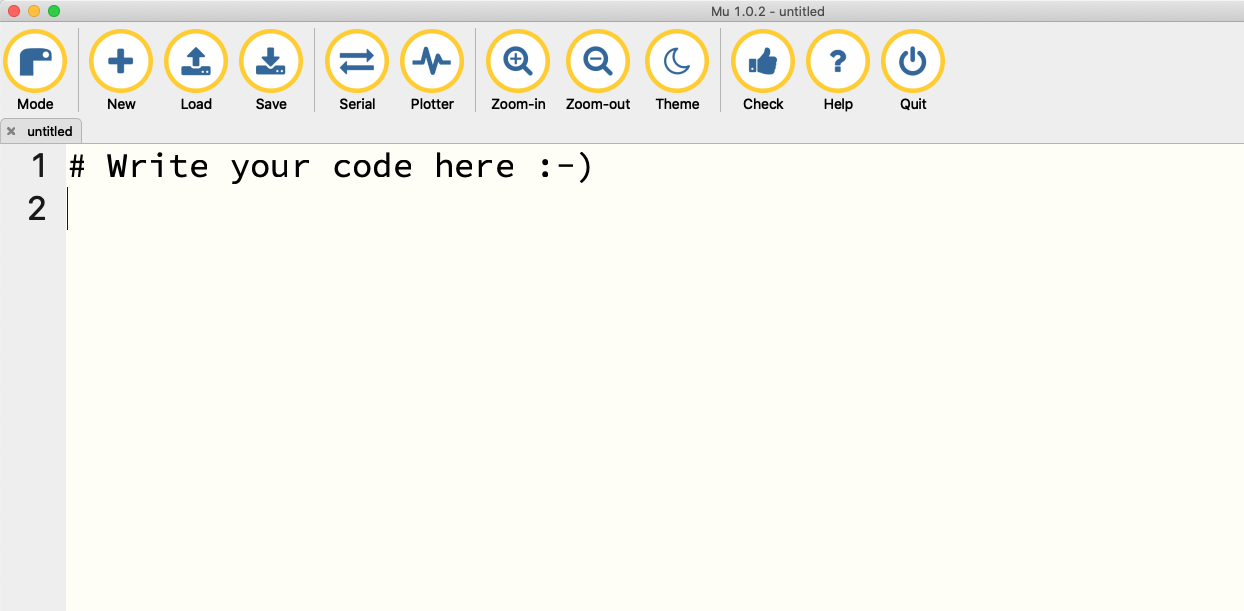
\includegraphics[width=1\linewidth]{images/03image1}

The first thing you'll notice is that it says \texttt{\#\ Write\ your\ code\ here\ :-)}. That's what's called a comment. Comments start with a \texttt{\#} and everything after it on that line will not be executed as code. So you can write whatever you want. You can also delete that line. Or keep it if you need the reminder. Either way, it's not going to do very much.

The first thing we're going to do to get started is we're going to make a tiny light blink. It's a good place to start because we're going to learn:

\begin{enumerate}
\def\labelenumi{\arabic{enumi}.}
\tightlist
\item
  How to write code in mu-editor.
\item
  How to save code in mu-editor.
\item
  How to move that code onto your board.
\item
  How to make a light blink.
\end{enumerate}

And in that order. Making a light blink isn't all that important, but the lessons learned doing it will be useful throughout.

This is the code we're going to use. DON'T JUST COPY AND PASTE IT. I want you to see a feature of mu-editor and other code editors. It's got many names, but it's aware of what you're typing and is going to try to make useful suggestions and offer up some simple documentation.

\begin{Shaded}
\begin{Highlighting}[]
\ImportTok{import}\NormalTok{ board}
\ImportTok{import}\NormalTok{ digitalio}
\ImportTok{import}\NormalTok{ time}

\NormalTok{led }\OperatorTok{=}\NormalTok{ digitalio.DigitalInOut(board.D13)}
\NormalTok{led.direction }\OperatorTok{=}\NormalTok{ digitalio.Direction.OUTPUT}

\ControlFlowTok{while} \VariableTok{True}\NormalTok{:}
\NormalTok{    led.value }\OperatorTok{=} \VariableTok{True}
\NormalTok{    time.sleep(.}\DecValTok{5}\NormalTok{)}
\NormalTok{    led.value }\OperatorTok{=} \VariableTok{False}
\NormalTok{    time.sleep(.}\DecValTok{5}\NormalTok{)}
\end{Highlighting}
\end{Shaded}

As you type, you should see suggestions like this:

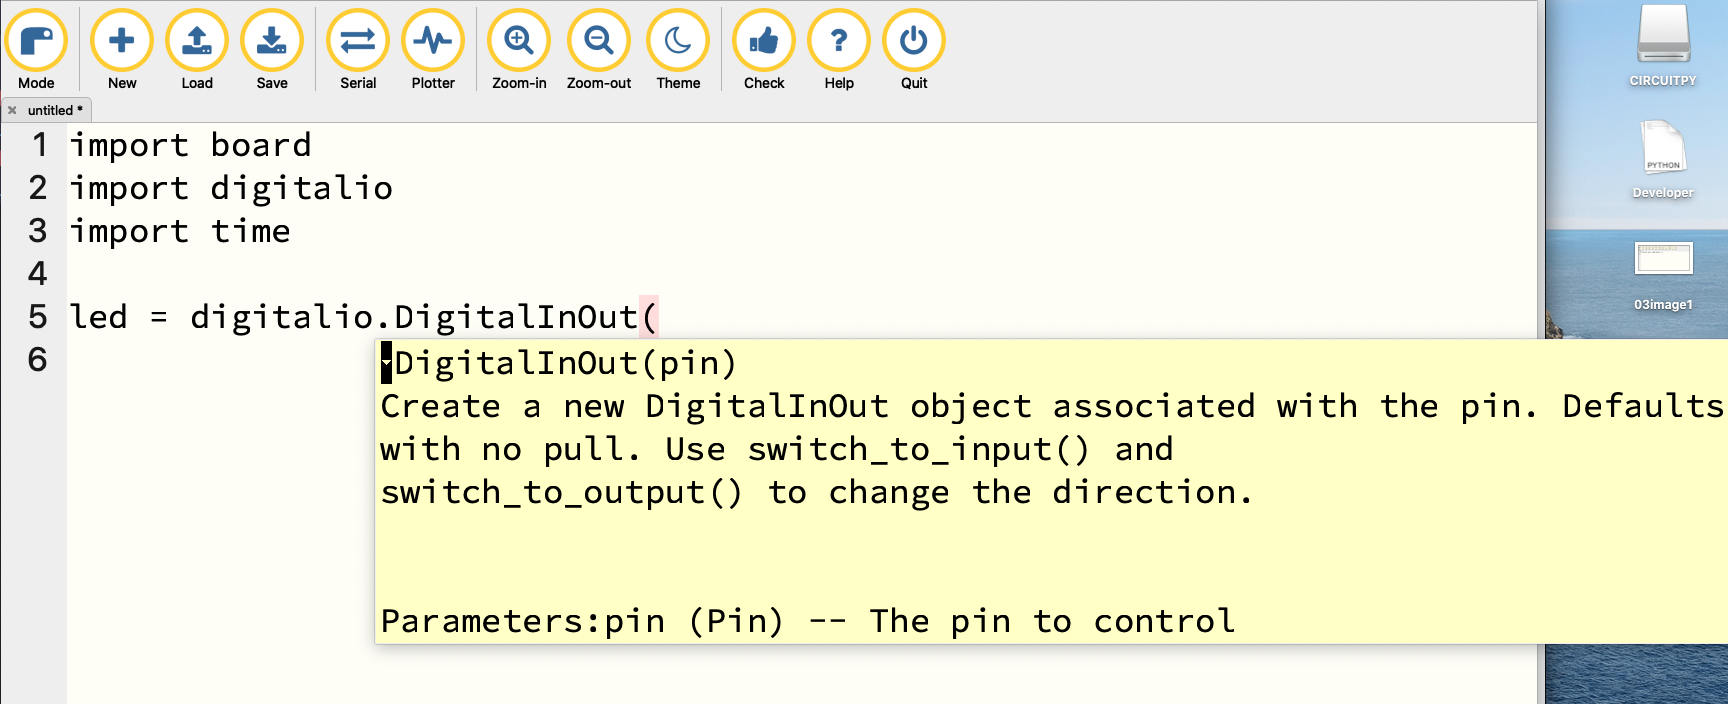
\includegraphics[width=1\linewidth]{images/03image2}

Let's walk through the code step by step.

First, the imports:

\begin{Shaded}
\begin{Highlighting}[]
\ImportTok{import}\NormalTok{ board}
\ImportTok{import}\NormalTok{ digitalio}
\ImportTok{import}\NormalTok{ time}
\end{Highlighting}
\end{Shaded}

In the previous chapter, we talked about external libraries that do common things. Here's where you start to see how deep that hole can go. These libraries, in order, give you access to the pieces and parts on your board, handles digital input and output to and from your board and gives you some tools to handle time.

The best practice for your code is to do your imports first, at the top.

Now, we do some setup.

\begin{Shaded}
\begin{Highlighting}[]
\NormalTok{led }\OperatorTok{=}\NormalTok{ digitalio.DigitalInOut(board.D13)}
\NormalTok{led.direction }\OperatorTok{=}\NormalTok{ digitalio.Direction.OUTPUT}
\end{Highlighting}
\end{Shaded}

The first thing we're going to do, is set up a variable called \texttt{led}. What \texttt{led} becomes is a Python thing called a Class. A Class is a generic description of a thing. In this case, the Class covers Digital Input and Output tools on your board. They're called pins. In this case, \texttt{led} is going to control digital pin 13 -- which we get from our \texttt{board} library. The D in front of the 13 means ``digital''. So \texttt{led} is going to control the input and output coming from digital pin 13.

The second thing is we need to set the direction of that input and output. This is easy when you're dealing with an led. It's a light. It's only output. So \texttt{led.direction} sets the direction of input or output to D13 to ``OUTPUT''.

Now, to the actual parts that make the board do things:

\begin{Shaded}
\begin{Highlighting}[]
\ControlFlowTok{while} \VariableTok{True}\NormalTok{:}
\NormalTok{    led.value }\OperatorTok{=} \VariableTok{True}
\NormalTok{    time.sleep(.}\DecValTok{5}\NormalTok{)}
\NormalTok{    led.value }\OperatorTok{=} \VariableTok{False}
\NormalTok{    time.sleep(.}\DecValTok{5}\NormalTok{)}
\end{Highlighting}
\end{Shaded}

This says \texttt{while\ True} -- without saying what is true or how to falsify it, so it's saying while the board is on -- set the led value to True, or on. Then, pause a half a second. Then turn it off. And pause half a second. Rinse and repeat forever.

Save this file and call it code.py

It has to be called code.py for it to work. When you load it onto the board, it will be looking for code.py.

Now take that code.py file and drag it into the CIRCUITPY drive.

Is a little red light blinking?

Now we can play with it a little.

Change the values in time.sleep. Save the file. Drag it over to your board. What happens?

\hypertarget{making-it-easier}{%
\section{Making it easier}\label{making-it-easier}}

How we just accomplished that is what could be described as the long way around doing this. We went to the very specific pieces and interacted with them. This will be an important pattern to rely on later, when we get to more complicated problems.

But in this case, it can be easier.

Adafruit has a library specific to their board, which connects things much more directly. Instead of having to connect to digitalIO and set things and name the specific pin on the board, Adafruit has made it easier by just creating a thing called red\_led.

\begin{Shaded}
\begin{Highlighting}[]
\ImportTok{import}\NormalTok{ time}
\ImportTok{from}\NormalTok{ adafruit_circuitplayground }\ImportTok{import}\NormalTok{ cp}
 
\ControlFlowTok{while} \VariableTok{True}\NormalTok{:}
\NormalTok{    cp.red_led }\OperatorTok{=} \VariableTok{True}
\NormalTok{    time.sleep(}\FloatTok{0.5}\NormalTok{)}
\NormalTok{    cp.red_led }\OperatorTok{=} \VariableTok{False}
\NormalTok{    time.sleep(}\FloatTok{0.5}\NormalTok{)}
\end{Highlighting}
\end{Shaded}

So this imports a thing called cp, which \ldots{} you can guess what that stands for \ldots{} and pretty much uses the while code from before to turn the red\_led on and off.

We can make it even easier with a little logic game.

\begin{Shaded}
\begin{Highlighting}[]
\ImportTok{import}\NormalTok{ time}
\ImportTok{from}\NormalTok{ adafruit_circuitplayground }\ImportTok{import}\NormalTok{ cp}

\ControlFlowTok{while} \VariableTok{True}\NormalTok{:}
\NormalTok{    cp.red_led }\OperatorTok{=} \KeywordTok{not}\NormalTok{ cp.red_led}
\NormalTok{    time.sleep(}\FloatTok{0.5}\NormalTok{)}
\end{Highlighting}
\end{Shaded}

But wait, how does this work? It works by exploiting what \texttt{cp.red\_led} can be. It can either be \texttt{True} or it can be \texttt{False}. The \texttt{not} in this case says set cp.red\_led to the other thing -- if it's \texttt{True}, make it \texttt{False} -- then pause a half a second. Then, if it's \texttt{False}, make it \texttt{True}, and pause. Repeat forever.

\hypertarget{more-fun-with-lights}{%
\section{More fun with lights}\label{more-fun-with-lights}}

Now that we've been introduced to Adafruit's board library, we can start to play with more things. Note there's much bigger lights than that tiny red led. Let's play with those.

Those lights are called NeoPixels, or in the Adafruit library, \texttt{pixels} for short. And we can \texttt{fill} those with whatever color we want.

How about red?

\begin{Shaded}
\begin{Highlighting}[]
\ImportTok{from}\NormalTok{ adafruit_circuitplayground }\ImportTok{import}\NormalTok{ cp}
 
\ControlFlowTok{while} \VariableTok{True}\NormalTok{:}
\NormalTok{    cp.pixels.fill((}\DecValTok{255}\NormalTok{, }\DecValTok{0}\NormalTok{, }\DecValTok{0}\NormalTok{)) }
\end{Highlighting}
\end{Shaded}

Or green?

\begin{Shaded}
\begin{Highlighting}[]
\ImportTok{from}\NormalTok{ adafruit_circuitplayground }\ImportTok{import}\NormalTok{ cp}
 
\ControlFlowTok{while} \VariableTok{True}\NormalTok{:}
\NormalTok{    cp.pixels.fill((}\DecValTok{0}\NormalTok{, }\DecValTok{255}\NormalTok{, }\DecValTok{0}\NormalTok{)) }
\end{Highlighting}
\end{Shaded}

Or blue?

\begin{Shaded}
\begin{Highlighting}[]
\ImportTok{from}\NormalTok{ adafruit_circuitplayground }\ImportTok{import}\NormalTok{ cp}
 
\ControlFlowTok{while} \VariableTok{True}\NormalTok{:}
\NormalTok{    cp.pixels.fill((}\DecValTok{0}\NormalTok{, }\DecValTok{0}\NormalTok{, }\DecValTok{255}\NormalTok{)) }
\end{Highlighting}
\end{Shaded}

You can make them blink.

\begin{Shaded}
\begin{Highlighting}[]
\ImportTok{import}\NormalTok{ time}
\ImportTok{from}\NormalTok{ adafruit_circuitplayground }\ImportTok{import}\NormalTok{ cp}
 
\ControlFlowTok{while} \VariableTok{True}\NormalTok{:}
\NormalTok{    cp.pixels.fill((}\DecValTok{0}\NormalTok{, }\DecValTok{0}\NormalTok{, }\DecValTok{255}\NormalTok{)) }
\NormalTok{    time.sleep(.}\DecValTok{5}\NormalTok{)}
\NormalTok{    cp.pixels.fill((}\DecValTok{0}\NormalTok{, }\DecValTok{0}\NormalTok{, }\DecValTok{0}\NormalTok{))}
\NormalTok{    time.sleep(.}\DecValTok{5}\NormalTok{)}
\end{Highlighting}
\end{Shaded}

You can light up just one of them.

\begin{Shaded}
\begin{Highlighting}[]
\ImportTok{from}\NormalTok{ adafruit_circuitplayground }\ImportTok{import}\NormalTok{ cp}
 
\ControlFlowTok{while} \VariableTok{True}\NormalTok{:}
\NormalTok{    cp.pixels[}\DecValTok{0}\NormalTok{] }\OperatorTok{=}\NormalTok{ (}\DecValTok{0}\NormalTok{, }\DecValTok{0}\NormalTok{, }\DecValTok{255}\NormalTok{) }
\end{Highlighting}
\end{Shaded}

Now, to understand how this works, you need to understand something about Python. Python counts in a weird way to everyone except programmers. Python starts counting at 0. So cp.pixels{[}0{]} is saying go to the first pixel and turn it blue. The rest are off.

\hypertarget{stretch-your-head}{%
\section{Stretch your head}\label{stretch-your-head}}

Before you run this, what do you think it's going to do?

\begin{Shaded}
\begin{Highlighting}[]
\ImportTok{import}\NormalTok{ time}
\ImportTok{from}\NormalTok{ adafruit_circuitplayground }\ImportTok{import}\NormalTok{ cp}
 
\ControlFlowTok{while} \VariableTok{True}\NormalTok{:}
\NormalTok{    cp.pixels[}\DecValTok{0}\NormalTok{] }\OperatorTok{=}\NormalTok{ (}\DecValTok{255}\NormalTok{, }\DecValTok{0}\NormalTok{, }\DecValTok{255}\NormalTok{) }
\NormalTok{    time.sleep(.}\DecValTok{1}\NormalTok{)}
\NormalTok{    cp.pixels[}\DecValTok{1}\NormalTok{] }\OperatorTok{=}\NormalTok{ (}\DecValTok{255}\NormalTok{, }\DecValTok{0}\NormalTok{, }\DecValTok{255}\NormalTok{)}
\NormalTok{    time.sleep(.}\DecValTok{1}\NormalTok{)}
\NormalTok{    cp.pixels[}\DecValTok{2}\NormalTok{] }\OperatorTok{=}\NormalTok{ (}\DecValTok{255}\NormalTok{, }\DecValTok{0}\NormalTok{, }\DecValTok{255}\NormalTok{)}
\NormalTok{    time.sleep(.}\DecValTok{1}\NormalTok{)}
\NormalTok{    cp.pixels[}\DecValTok{3}\NormalTok{] }\OperatorTok{=}\NormalTok{ (}\DecValTok{255}\NormalTok{, }\DecValTok{0}\NormalTok{, }\DecValTok{255}\NormalTok{)}
\NormalTok{    time.sleep(.}\DecValTok{1}\NormalTok{)}
\NormalTok{    cp.pixels[}\DecValTok{4}\NormalTok{] }\OperatorTok{=}\NormalTok{ (}\DecValTok{255}\NormalTok{, }\DecValTok{0}\NormalTok{, }\DecValTok{255}\NormalTok{)}
\NormalTok{    time.sleep(.}\DecValTok{1}\NormalTok{)}
\NormalTok{    cp.pixels[}\DecValTok{5}\NormalTok{] }\OperatorTok{=}\NormalTok{ (}\DecValTok{255}\NormalTok{, }\DecValTok{0}\NormalTok{, }\DecValTok{255}\NormalTok{)}
\NormalTok{    time.sleep(.}\DecValTok{1}\NormalTok{)}
\NormalTok{    cp.pixels[}\DecValTok{6}\NormalTok{] }\OperatorTok{=}\NormalTok{ (}\DecValTok{255}\NormalTok{, }\DecValTok{0}\NormalTok{, }\DecValTok{255}\NormalTok{)}
\NormalTok{    time.sleep(.}\DecValTok{1}\NormalTok{)}
\NormalTok{    cp.pixels[}\DecValTok{7}\NormalTok{] }\OperatorTok{=}\NormalTok{ (}\DecValTok{255}\NormalTok{, }\DecValTok{0}\NormalTok{, }\DecValTok{255}\NormalTok{)}
\NormalTok{    time.sleep(.}\DecValTok{1}\NormalTok{)}
\NormalTok{    cp.pixels[}\DecValTok{8}\NormalTok{] }\OperatorTok{=}\NormalTok{ (}\DecValTok{255}\NormalTok{, }\DecValTok{0}\NormalTok{, }\DecValTok{255}\NormalTok{)}
\NormalTok{    time.sleep(.}\DecValTok{1}\NormalTok{)}
\NormalTok{    cp.pixels[}\DecValTok{9}\NormalTok{] }\OperatorTok{=}\NormalTok{ (}\DecValTok{255}\NormalTok{, }\DecValTok{0}\NormalTok{, }\DecValTok{255}\NormalTok{)}
\NormalTok{    time.sleep(.}\DecValTok{1}\NormalTok{)}
\NormalTok{    cp.pixels.fill((}\DecValTok{0}\NormalTok{, }\DecValTok{0}\NormalTok{, }\DecValTok{0}\NormalTok{))}
\NormalTok{    time.sleep(.}\DecValTok{1}\NormalTok{)}
\NormalTok{    cp.pixels.fill((}\DecValTok{255}\NormalTok{, }\DecValTok{0}\NormalTok{, }\DecValTok{255}\NormalTok{))}
\NormalTok{    time.sleep(.}\DecValTok{1}\NormalTok{)}
\NormalTok{    cp.pixels.fill((}\DecValTok{0}\NormalTok{, }\DecValTok{0}\NormalTok{, }\DecValTok{0}\NormalTok{))}
\NormalTok{    time.sleep(.}\DecValTok{1}\NormalTok{)}
\NormalTok{    cp.pixels.fill((}\DecValTok{255}\NormalTok{, }\DecValTok{0}\NormalTok{, }\DecValTok{255}\NormalTok{))}
\NormalTok{    time.sleep(.}\DecValTok{1}\NormalTok{)}
\NormalTok{    cp.pixels.fill((}\DecValTok{0}\NormalTok{, }\DecValTok{0}\NormalTok{, }\DecValTok{0}\NormalTok{))}
\NormalTok{    time.sleep(.}\DecValTok{1}\NormalTok{)}
\NormalTok{    cp.pixels.fill((}\DecValTok{255}\NormalTok{, }\DecValTok{0}\NormalTok{, }\DecValTok{255}\NormalTok{))}
\NormalTok{    time.sleep(.}\DecValTok{1}\NormalTok{)}
\NormalTok{    cp.pixels.fill((}\DecValTok{0}\NormalTok{, }\DecValTok{0}\NormalTok{, }\DecValTok{0}\NormalTok{))}
\NormalTok{    time.sleep(.}\DecValTok{1}\NormalTok{)}
\end{Highlighting}
\end{Shaded}

The RGB value of 255, 0, 255 is full red and full blue -- Purple. So it turns on the first, turns on the second, turns on the third and so on until all of them are lit up, turns them all off and on three times and repeats. All I did to make this? Copy, paste, change a value and repeat.

\hypertarget{light-sensing-and-what-numbers-mean}{%
\chapter{Light sensing and what numbers mean}\label{light-sensing-and-what-numbers-mean}}

Up to now, we've been building toward sensing things. We've learned a little Python, wrote some code and make some lights turn on and off. But journalism isn't about blinking lights, it's about learning things about your environment and reporting them to others.

On your board are three sensors we're going to use in the next three chapters: The light sensor, the temperature sensor and the sound sensor. If you look at your Circuit Playground, you can find them by their symbols.

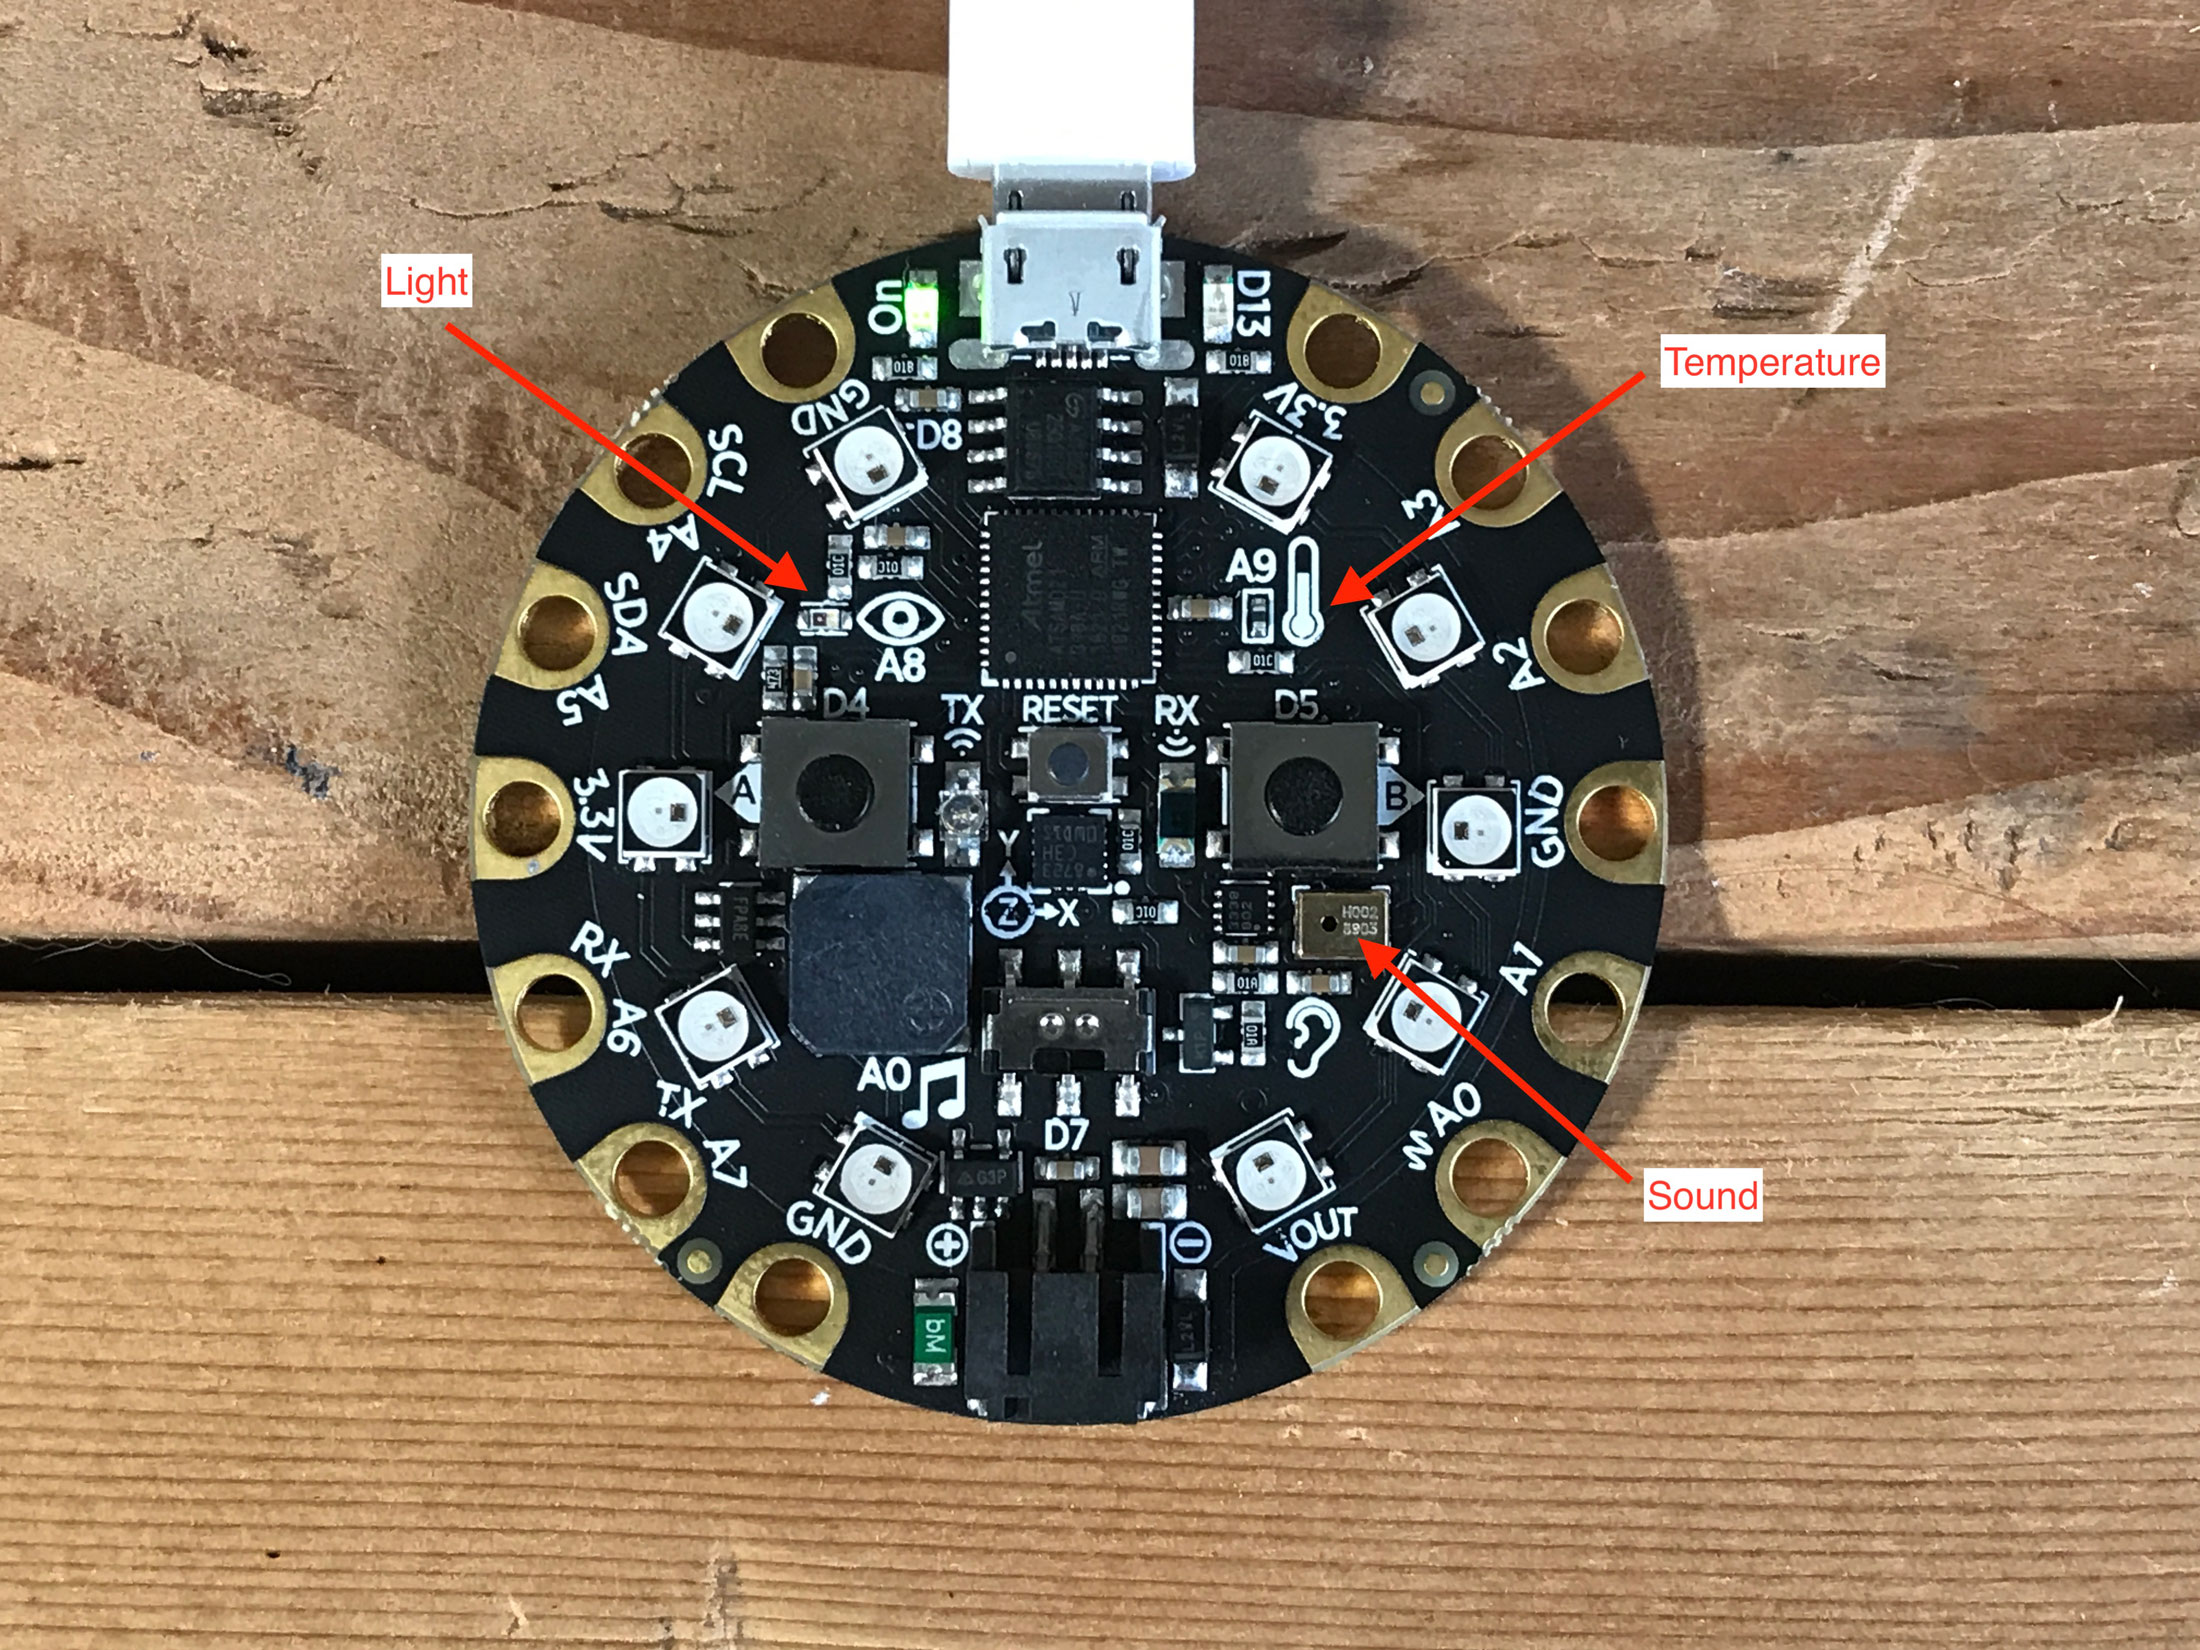
\includegraphics[width=1\linewidth]{images/04image1}
We'll start with light. Maybe your story needs to know how bright or dark it is in a place for periods of time. The light sensor on board can tell you on a continuous scale what level of light there is. According to \href{https://cdn-learn.adafruit.com/downloads/pdf/adafruit-circuit-playground-express.pdf}{Adafruit's documentation}, the numbers range from from 0 -- complete darkness -- to 1023. Since the light sensor is an analog sensor, those are voltage measures.

Now, here's where sensor journalism starts to get a little more difficult.

First, let's get some code going to illustrate this.

\begin{Shaded}
\begin{Highlighting}[]
\ImportTok{import}\NormalTok{ time}
\ImportTok{from}\NormalTok{ adafruit_circuitplayground }\ImportTok{import}\NormalTok{ cp}
 
\ControlFlowTok{while} \VariableTok{True}\NormalTok{:}
    \BuiltInTok{print}\NormalTok{(}\StringTok{"Light:"}\NormalTok{, cp.light)}
\NormalTok{    time.sleep(}\DecValTok{1}\NormalTok{)}
\end{Highlighting}
\end{Shaded}

Save that to your board, and then click on the Serial button in the toolbar.

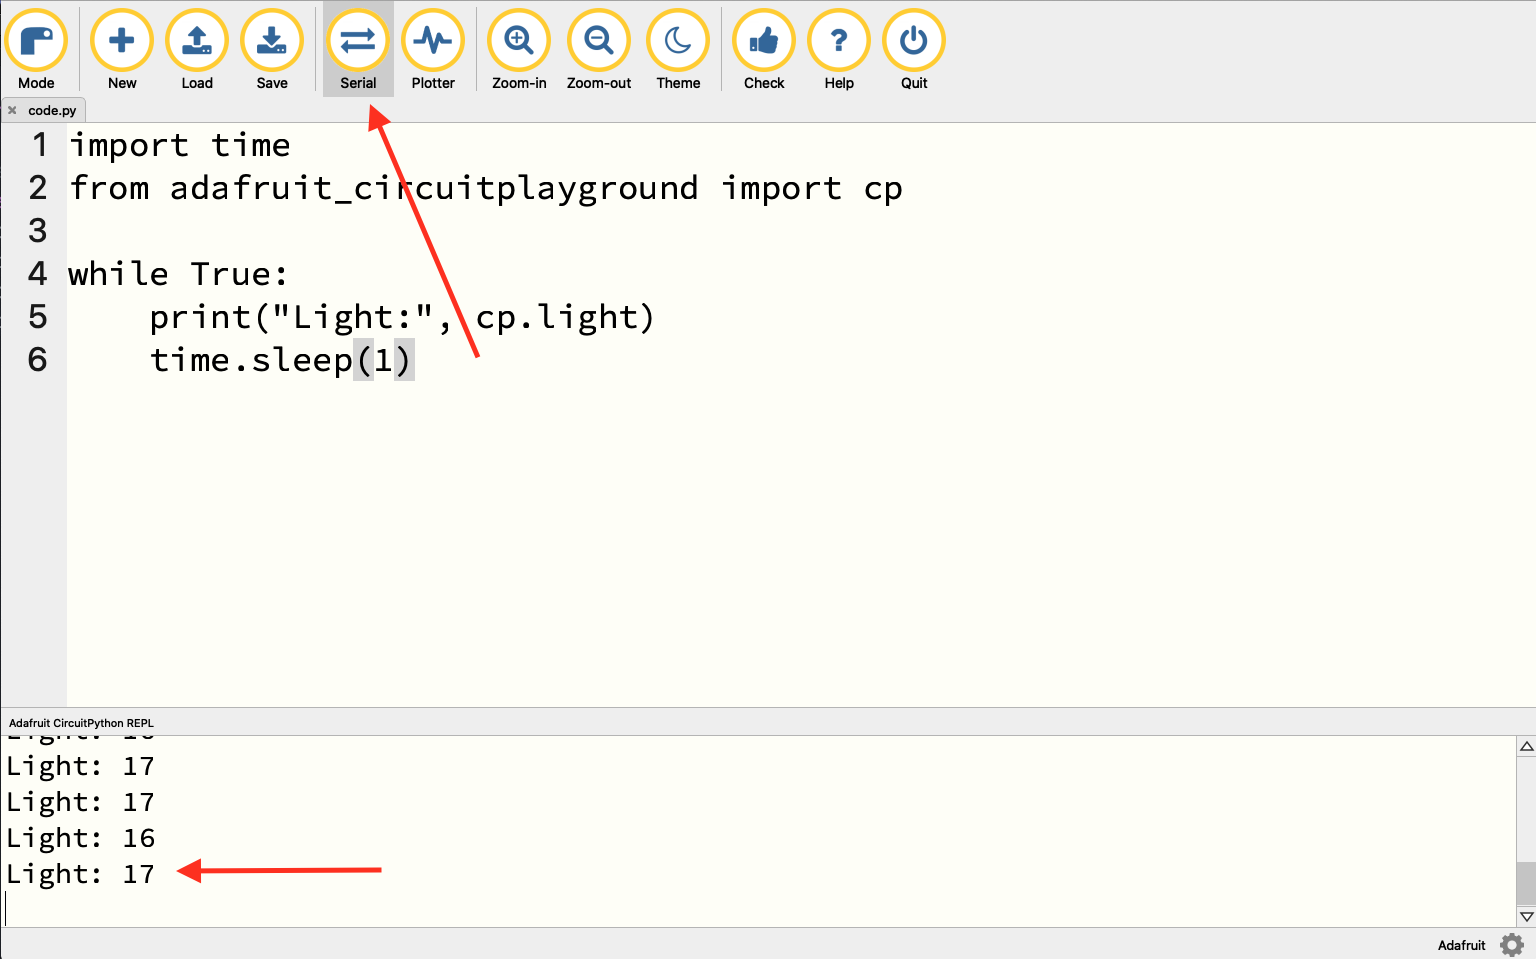
\includegraphics[width=1\linewidth]{images/04image2}

So you can see, my office is a little bit dim. I'm in a basement office with a half window next to me, but that window is partially underneath a deck, so the amount of sun coming in is indirect. So my light reading is 17. Now watch what happens when I bring in a lamp with a 100 watt equivalent LED in it.

With that very bright light -- so bright you can't look at it directly without pain -- the number goes up to 320.

I walked outside on a sunny summer day without a cloud in the sky and it topped out at 321.

But what does that mean? What does 321 mean? And if direct bright light is 321, what is 1023?

Light is measured in Lux, but would you know the difference between 1500 and 10000 Lux?

As journalists, we love numbers, but sometimes the number isn't that important. Maybe what's better here is to know that 320 is very bright and less than 50 is dim and maybe we come up with some categories in between. Ask yourself: do you need an exact number? Is that number meaningful? Or is it enough to just know the difference between very bright, bright, dim and dark?

\hypertarget{not-to-feed-your-love-of-numbers-but}{%
\section{Not to feed your love of numbers, but \ldots{}}\label{not-to-feed-your-love-of-numbers-but}}

You may have noticed, when you clicked the Serial button, that's there's a Plotter button.

To use the plotter, we have to have something in Python called a tuple. A tuple is a kind of data that has two parts. You create them with parenthesis, and you separate the two elements of data in the tuple with a comma. To use the plotter, you're code has to produce a tuple. Here's one way.

\begin{Shaded}
\begin{Highlighting}[]
\ImportTok{import}\NormalTok{ time}
\ImportTok{from}\NormalTok{ adafruit_circuitplayground }\ImportTok{import}\NormalTok{ cp}
 
\ControlFlowTok{while} \VariableTok{True}\NormalTok{:}
    \BuiltInTok{print}\NormalTok{((cp.light,))}
\NormalTok{    time.sleep(}\DecValTok{1}\NormalTok{)}
\end{Highlighting}
\end{Shaded}

Save that to your board and click the Plotter button. You should now get a line chart showing change over time.

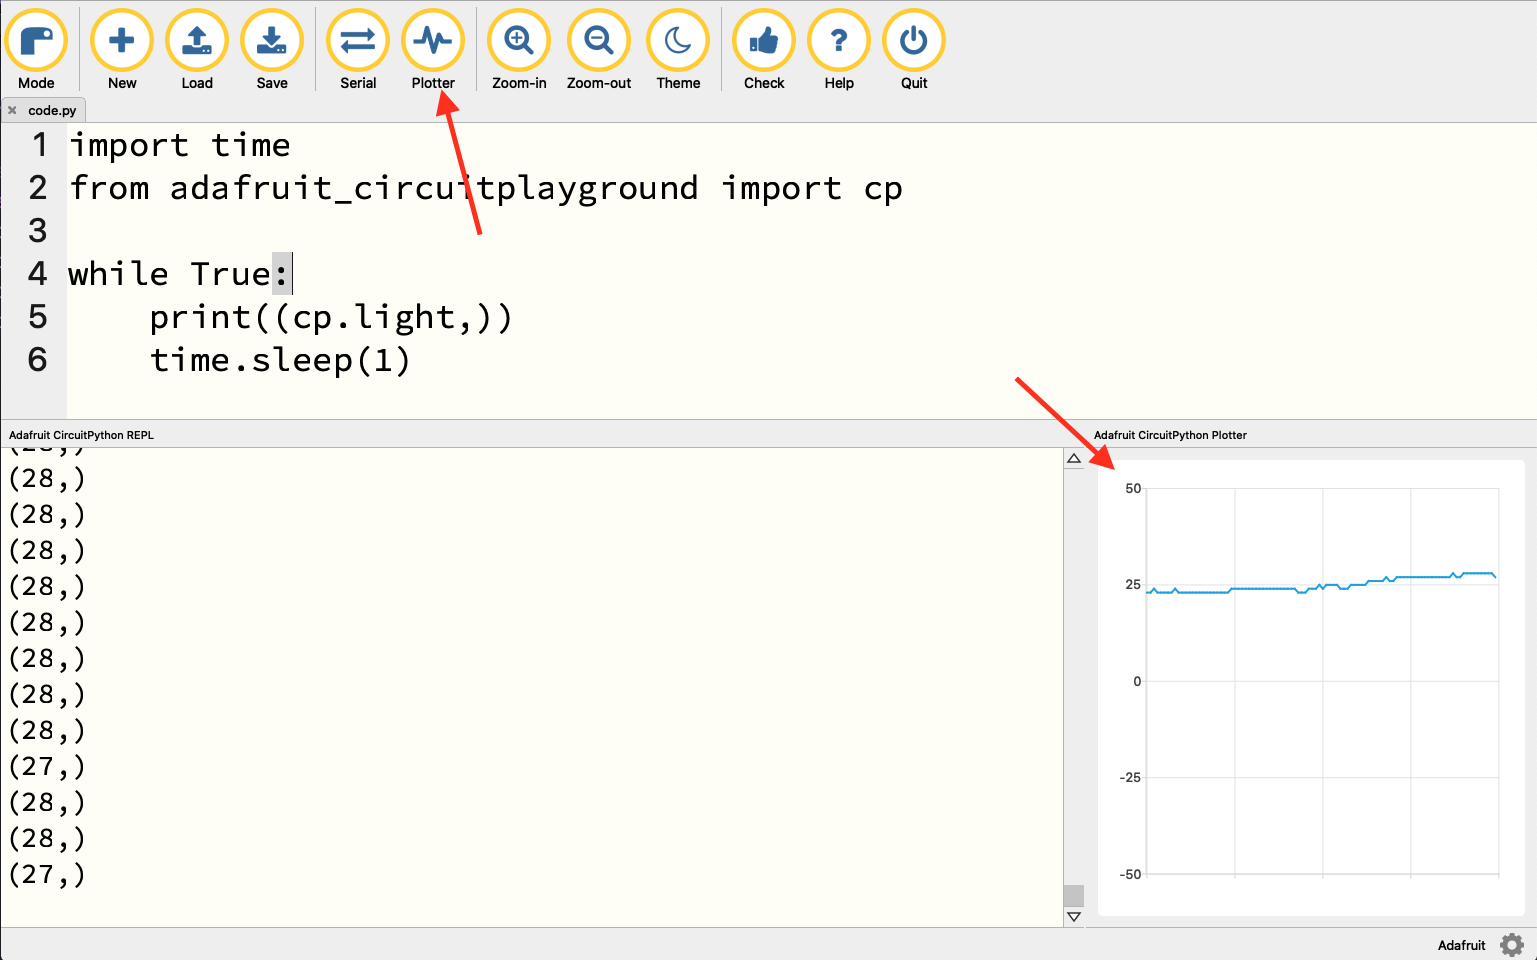
\includegraphics[width=1\linewidth]{images/04image3}

And while that's cool to see, what does 27 mean? Something to think deeply about before you go forward with your sensor journalism project.

\hypertarget{temperature-and-accuracy}{%
\chapter{Temperature and accuracy}\label{temperature-and-accuracy}}

Another sensor on the board is the temperature sensor. Unlike the light sensor, the data it returns is very easy to understand: It's the temperature in Celcius.

\begin{Shaded}
\begin{Highlighting}[]
\ImportTok{import}\NormalTok{ time}
\ImportTok{from}\NormalTok{ adafruit_circuitplayground }\ImportTok{import}\NormalTok{ cp}
 
\ControlFlowTok{while} \VariableTok{True}\NormalTok{:}
    \BuiltInTok{print}\NormalTok{(cp.temperature)}
\NormalTok{    time.sleep(}\DecValTok{1}\NormalTok{)}
\end{Highlighting}
\end{Shaded}

If you save that to your board and look at the Serial output, you'll see numbers probably around 24. That's 24 degrees Celcius. You can add things to the print statement to help you out.

\begin{Shaded}
\begin{Highlighting}[]
\ImportTok{import}\NormalTok{ time}
\ImportTok{from}\NormalTok{ adafruit_circuitplayground }\ImportTok{import}\NormalTok{ cp}
 
\ControlFlowTok{while} \VariableTok{True}\NormalTok{:}
    \BuiltInTok{print}\NormalTok{(cp.temperature, }\StringTok{"C"}\NormalTok{)}
\NormalTok{    time.sleep(}\DecValTok{1}\NormalTok{)}
\end{Highlighting}
\end{Shaded}

Remember in Chapter 2 when we converted C to F? Let's bring that back.

\begin{Shaded}
\begin{Highlighting}[]
\ImportTok{import}\NormalTok{ time}
\ImportTok{from}\NormalTok{ adafruit_circuitplayground }\ImportTok{import}\NormalTok{ cp}

\KeywordTok{def}\NormalTok{ convert(temp):}
\NormalTok{    fahren }\OperatorTok{=}\NormalTok{ (temp }\OperatorTok{*} \FloatTok{1.8}\NormalTok{) }\OperatorTok{+} \DecValTok{32} 
    \BuiltInTok{print}\NormalTok{(fahren) }

\ControlFlowTok{while} \VariableTok{True}\NormalTok{:}
\NormalTok{    convert(cp.temperature)}
\NormalTok{    time.sleep(}\DecValTok{1}\NormalTok{)}
\end{Highlighting}
\end{Shaded}

Now that is telling me that my office is about 77.8 degrees Fahrenheit. Now I'm notoriously Dad Energy on this -- air conditioning is expensive, so I don't care if you're warm -- but my basement office is quite cool. It isn't 77.8.

So what is it?

That raises questions about how accurate are your sensors. The truth is this is one place where you get what you pay for. Do you need extremely accurate temperature readings because any change will cost your business money? Then you spend whatever it takes to get the most accurate sensor. Are you making a journalism project where a little fuzziness is not a huge deal? Then the sensor isn't going to cost as much.

But can we make this better without spending more money? We can.

\hypertarget{turning-down-the-noise}{%
\section{Turning down the noise}\label{turning-down-the-noise}}

When planning a sensor journalism project, there's several questions you're going to have to answer given your requirements and given your available equipment.

Two critical questions will be:

\begin{enumerate}
\def\labelenumi{\arabic{enumi}.}
\tightlist
\item
  How accurate does the measurement have to be? Is good enough good enough?
\item
  How precise does the measurement need to be?
\end{enumerate}

For example, my readings are saying things like 78.6844. Do we really need four digits of precision? Can you tell the difference between 78.6844 and 78.6855? Do people talk about temperature with decimals?

And notice that the sensor is sensitive enough that the temperature goes up and down with each reading, no matter how frequently you ask for it. We've got it set for every second. Do micro differences in temperature every second matter?

There are some things we can do in code to deal with these questions.

First, we can average a collection of temperature readings to smooth it out. To do this, we're going to create an empty list, then populate it with readings every second. Then, when we hit a threshold level -- we'll start with 5 -- we'll average them together. We'll clear out the list, and start it all over again.

\begin{Shaded}
\begin{Highlighting}[]
\ImportTok{import}\NormalTok{ time}
\ImportTok{from}\NormalTok{ adafruit_circuitplayground }\ImportTok{import}\NormalTok{ cp}

\NormalTok{temps }\OperatorTok{=}\NormalTok{ [] }\CommentTok{# here's the empty list}

\KeywordTok{def}\NormalTok{ convert(temp):}
\NormalTok{    fahren }\OperatorTok{=}\NormalTok{ (temp }\OperatorTok{*} \FloatTok{1.8}\NormalTok{) }\OperatorTok{+} \DecValTok{32} 
    \ControlFlowTok{return}\NormalTok{ fahren }

\ControlFlowTok{while} \VariableTok{True}\NormalTok{: }\CommentTok{# do this forever}
    \ControlFlowTok{while} \BuiltInTok{len}\NormalTok{(temps) }\OperatorTok{!=} \DecValTok{5}\NormalTok{: }\CommentTok{# while the number of readings in our list isn't 5 }
\NormalTok{        temps.append(convert(cp.temperature)) }\CommentTok{# append each temperature reading in Fahrenheit to the list}
\NormalTok{        time.sleep(}\DecValTok{1}\NormalTok{) }\CommentTok{# wait a second and repeat it again}
    \BuiltInTok{print}\NormalTok{(}\BuiltInTok{sum}\NormalTok{(temps)}\OperatorTok{/}\DecValTok{5}\NormalTok{) }\CommentTok{# once the while loop breaks, we'll add them up and divide by 5 and print it}
\NormalTok{    temps.clear() }\CommentTok{# empty the list so the inner while loop can start again}
\end{Highlighting}
\end{Shaded}

That, by itself, smooths out the readings some.

But what else can we do?

Let's eliminate the decimal points.

\begin{Shaded}
\begin{Highlighting}[]
\ImportTok{import}\NormalTok{ time}
\ImportTok{from}\NormalTok{ adafruit_circuitplayground }\ImportTok{import}\NormalTok{ cp}

\NormalTok{temps }\OperatorTok{=}\NormalTok{ []}

\KeywordTok{def}\NormalTok{ convert(temp):}
\NormalTok{    fahren }\OperatorTok{=}\NormalTok{ (temp }\OperatorTok{*} \FloatTok{1.8}\NormalTok{) }\OperatorTok{+} \DecValTok{32} 
    \ControlFlowTok{return}\NormalTok{ fahren }

\ControlFlowTok{while} \VariableTok{True}\NormalTok{:}
    \ControlFlowTok{while} \BuiltInTok{len}\NormalTok{(temps) }\OperatorTok{!=} \DecValTok{5}\NormalTok{:}
\NormalTok{        temps.append(convert(cp.temperature))}
\NormalTok{        time.sleep(}\DecValTok{1}\NormalTok{)}
\NormalTok{    avg }\OperatorTok{=} \BuiltInTok{sum}\NormalTok{(temps)}\OperatorTok{/}\DecValTok{5}
    \BuiltInTok{print}\NormalTok{(}\StringTok{"%.0f"} \OperatorTok{%} \BuiltInTok{round}\NormalTok{(avg, }\DecValTok{0}\NormalTok{)) }\CommentTok{# the first formats the output to have zero digits, the second part rounds}
\NormalTok{    temps.clear()}
\end{Highlighting}
\end{Shaded}

Now my sensor says its between 78 and 79 in my office, which is much more like how we are accustomed to talking about temperature. But it is right?

\hypertarget{low-cost-validation-and-calibration}{%
\section{Low cost validation and calibration}\label{low-cost-validation-and-calibration}}

As I said earlier, I'm pretty Dad Energy about the temperature in my house. But a basement office is generally cooler than the rest of the house -- so much so that I have the vents closed so as to not add more cold air in the room. So how is it telling me that my office is 79 when the thermostat upstairs is set at 76?

One thing we can do is compare our sensor to an external sensor and compare. How different is our measurement from a better sensor.

My house has an Ecobee Smart Thermostat system and I've got a movable remote temperature sensor. Since I trust it to cool my house, I'm going to trust it here to give a better reading on the temperature in my office.

So what does the sensor say it is? 75.

The sensor, averaging five readings and averaging them together before rounding them to the nearest whole degree -- now reads 78.

Simple solution? Knock three off our sensor reading to make it closer to the external sensor, which much more conforms with my understanding of what it actually feels like in my office.

Your situation is going to be different, so you'll need an external temperature gauge to validate your sensor output and adjust accordingly. But here's my code.

\begin{Shaded}
\begin{Highlighting}[]
\ImportTok{import}\NormalTok{ time}
\ImportTok{from}\NormalTok{ adafruit_circuitplayground }\ImportTok{import}\NormalTok{ cp}

\NormalTok{temps }\OperatorTok{=}\NormalTok{ []}

\KeywordTok{def}\NormalTok{ convert(temp):}
\NormalTok{    fahren }\OperatorTok{=}\NormalTok{ (temp }\OperatorTok{*} \FloatTok{1.8}\NormalTok{) }\OperatorTok{+} \DecValTok{32} 
    \ControlFlowTok{return}\NormalTok{ fahren }

\ControlFlowTok{while} \VariableTok{True}\NormalTok{:}
    \ControlFlowTok{while} \BuiltInTok{len}\NormalTok{(temps) }\OperatorTok{!=} \DecValTok{5}\NormalTok{:}
\NormalTok{        temps.append(convert(cp.temperature))}
\NormalTok{        time.sleep(}\DecValTok{1}\NormalTok{)}
\NormalTok{    avg }\OperatorTok{=}\NormalTok{ (}\BuiltInTok{sum}\NormalTok{(temps)}\OperatorTok{/}\DecValTok{5}\NormalTok{) }\OperatorTok{-} \DecValTok{3} \CommentTok{# the - 3 is the adjustment to be as close to reality as we can get.}
    \BuiltInTok{print}\NormalTok{(}\StringTok{"%.0f"} \OperatorTok{%} \BuiltInTok{round}\NormalTok{(avg, }\DecValTok{0}\NormalTok{)) }
\NormalTok{    temps.clear()}
\end{Highlighting}
\end{Shaded}

\hypertarget{sound}{%
\chapter{Sound}\label{sound}}

\begin{Shaded}
\begin{Highlighting}[]
\ImportTok{import}\NormalTok{ array}
\ImportTok{import}\NormalTok{ math}
\ImportTok{import}\NormalTok{ time}

\ImportTok{import}\NormalTok{ audiobusio}
\ImportTok{import}\NormalTok{ board}


\KeywordTok{def}\NormalTok{ mean(values):}
    \ControlFlowTok{return} \BuiltInTok{sum}\NormalTok{(values) }\OperatorTok{/} \BuiltInTok{len}\NormalTok{(values)}


\KeywordTok{def}\NormalTok{ normalized_rms(values):}
\NormalTok{    minbuf }\OperatorTok{=} \BuiltInTok{int}\NormalTok{(mean(values))}
\NormalTok{    sum_of_samples }\OperatorTok{=} \BuiltInTok{sum}\NormalTok{(}
        \BuiltInTok{float}\NormalTok{(sample }\OperatorTok{-}\NormalTok{ minbuf) }\OperatorTok{*}\NormalTok{ (sample }\OperatorTok{-}\NormalTok{ minbuf)}
        \ControlFlowTok{for}\NormalTok{ sample }\KeywordTok{in}\NormalTok{ values}
\NormalTok{    )}

    \ControlFlowTok{return}\NormalTok{ math.sqrt(sum_of_samples }\OperatorTok{/} \BuiltInTok{len}\NormalTok{(values))}


\NormalTok{mic }\OperatorTok{=}\NormalTok{ audiobusio.PDMIn(}
\NormalTok{    board.MICROPHONE_CLOCK,}
\NormalTok{    board.MICROPHONE_DATA,}
\NormalTok{    sample_rate}\OperatorTok{=}\DecValTok{16000}\NormalTok{,}
\NormalTok{    bit_depth}\OperatorTok{=}\DecValTok{16}
\NormalTok{)}
\NormalTok{samples }\OperatorTok{=}\NormalTok{ array.array(}\StringTok{'H'}\NormalTok{, [}\DecValTok{0}\NormalTok{] }\OperatorTok{*} \DecValTok{160}\NormalTok{)}
\NormalTok{mic.record(samples, }\BuiltInTok{len}\NormalTok{(samples))}

\ControlFlowTok{while} \VariableTok{True}\NormalTok{:}
\NormalTok{    mic.record(samples, }\BuiltInTok{len}\NormalTok{(samples))}
\NormalTok{    magnitude }\OperatorTok{=}\NormalTok{ normalized_rms(samples)}
    \BuiltInTok{print}\NormalTok{(((magnitude),))}
\NormalTok{    time.sleep(}\DecValTok{1}\NormalTok{)}
\end{Highlighting}
\end{Shaded}

\hypertarget{counting-with-buttons}{%
\chapter{Counting with buttons}\label{counting-with-buttons}}

\begin{Shaded}
\begin{Highlighting}[]
\ImportTok{import}\NormalTok{ time}
\ImportTok{from}\NormalTok{ adafruit_circuitplayground }\ImportTok{import}\NormalTok{ cp}

\NormalTok{count }\OperatorTok{=} \DecValTok{0}

\ControlFlowTok{while} \VariableTok{True}\NormalTok{:}
    \ControlFlowTok{if}\NormalTok{ cp.button_b:}
\NormalTok{        count }\OperatorTok{+=} \DecValTok{1}
\NormalTok{        cp.pixels[}\DecValTok{9}\NormalTok{] }\OperatorTok{=}\NormalTok{ (}\DecValTok{0}\NormalTok{, }\DecValTok{255}\NormalTok{, }\DecValTok{0}\NormalTok{)}
\NormalTok{        time.sleep(.}\DecValTok{2}\NormalTok{)}
        \BuiltInTok{print}\NormalTok{(count)}
\NormalTok{        cp.pixels[}\DecValTok{9}\NormalTok{] }\OperatorTok{=}\NormalTok{ (}\DecValTok{0}\NormalTok{, }\DecValTok{0}\NormalTok{, }\DecValTok{0}\NormalTok{)}
    \ControlFlowTok{if}\NormalTok{ cp.button_a:}
\NormalTok{        count }\OperatorTok{-=} \DecValTok{1}
\NormalTok{        cp.pixels[}\DecValTok{0}\NormalTok{] }\OperatorTok{=}\NormalTok{ (}\DecValTok{255}\NormalTok{, }\DecValTok{0}\NormalTok{, }\DecValTok{0}\NormalTok{)}
\NormalTok{        time.sleep(.}\DecValTok{2}\NormalTok{)}
        \BuiltInTok{print}\NormalTok{(count)}
\NormalTok{        cp.pixels[}\DecValTok{0}\NormalTok{] }\OperatorTok{=}\NormalTok{ (}\DecValTok{0}\NormalTok{, }\DecValTok{0}\NormalTok{, }\DecValTok{0}\NormalTok{)}
\end{Highlighting}
\end{Shaded}

\hypertarget{touch}{%
\chapter{Touch}\label{touch}}

\end{document}
